%%%%%%%%%%%%%%%%%%%%%%%%%%%%%%%%%%%%%%%%%%%%%%%%%%%%%%%%%%%%%%%%%%%%%%%%%%%%%%%%%%
%%% Crawl Gait
%%% 
%%%
%%%%%%%%%%%%%%%%%%%%%%%%%%%%%%%%%%%%%%%%%%%%%%%%%%%%%%%%%%%%%%%%%%%%%%%%%%%%%%%%%%
\chapter{Crawl Gait Results} \label{ch:results_crawl_gait}

% The structure of this chapter needs revision.

% What do we have to talk about here?
% Well, I suppose the point of this chapter is to present how well the algorithm worked.
% What is there to present?
% I suppose it should be shown that the crawl gait does indeed crawl the robot,
% as that is not necessarily assumed in the chapter explaining the gait.
% Some things you might want to know:
% How fast did the robot go?
% How high?
% What was the torque usage?

Crap I have to say about crawling.

PUT A PROJECTED PROFILE PICTURE HERE FOR THE INTRO.

THESE ARE ALL DONE WITH THE TRIVIAL TRIPLET PARAMETERS.

Explain the gait and it's parameters.

Explain the different experimental setups.

Explain that the point of this setup is to show that the crawl gait is very low profile.
\begin{figure}
  \vspace*{0.02in}
  \centerline{
    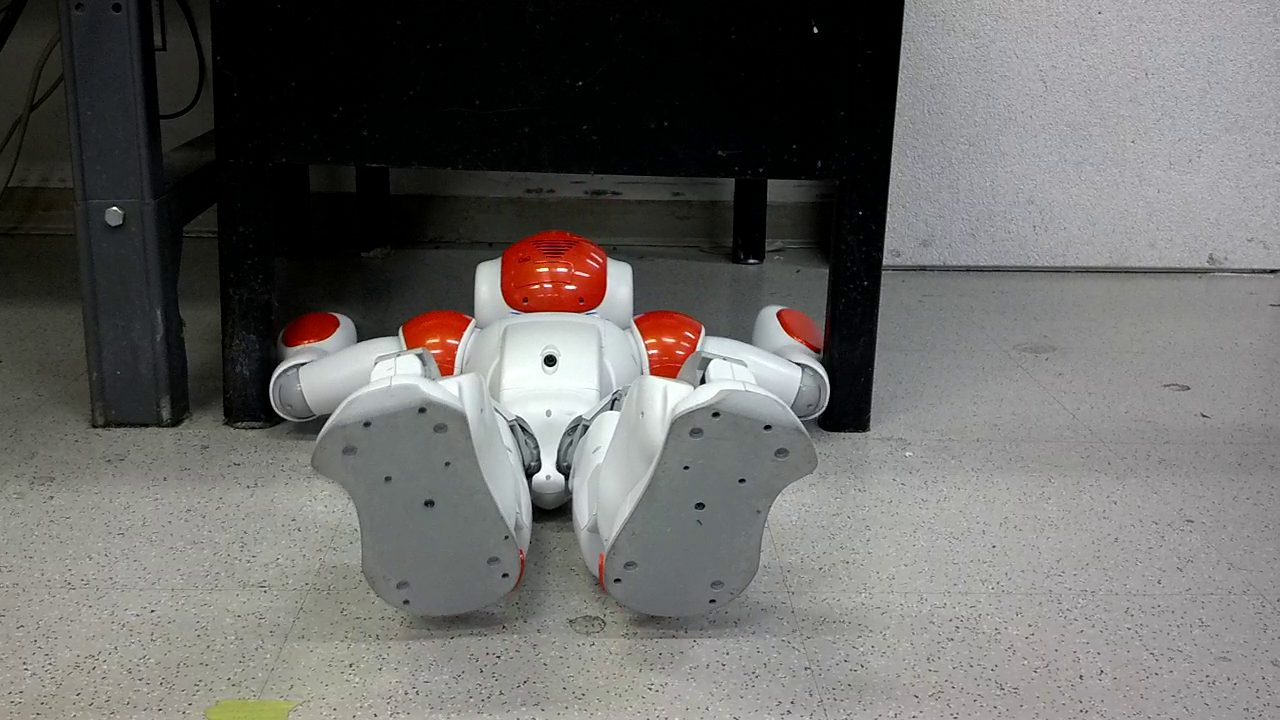
\includegraphics[width=0.25\textwidth]{crawl/under_table/14s.png}
    \includegraphics[width=0.25\textwidth]{crawl/under_table/18s.png}
    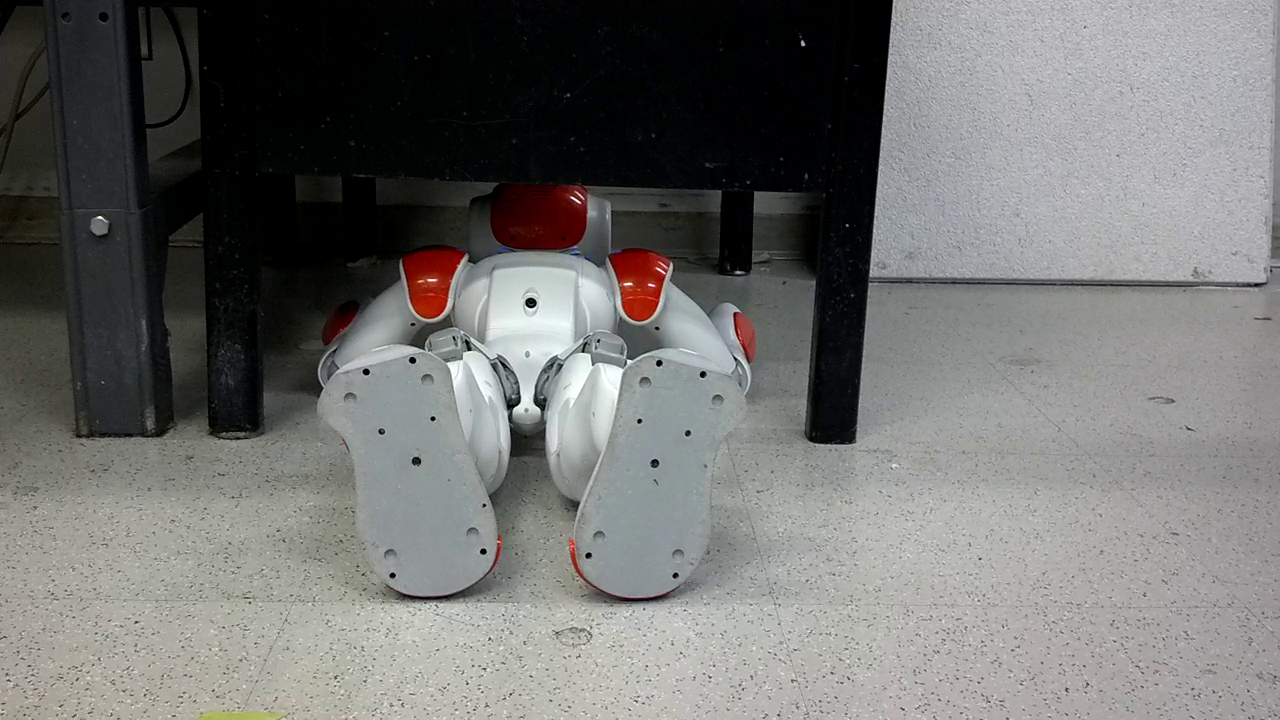
\includegraphics[width=0.25\textwidth]{crawl/under_table/19s.png}
    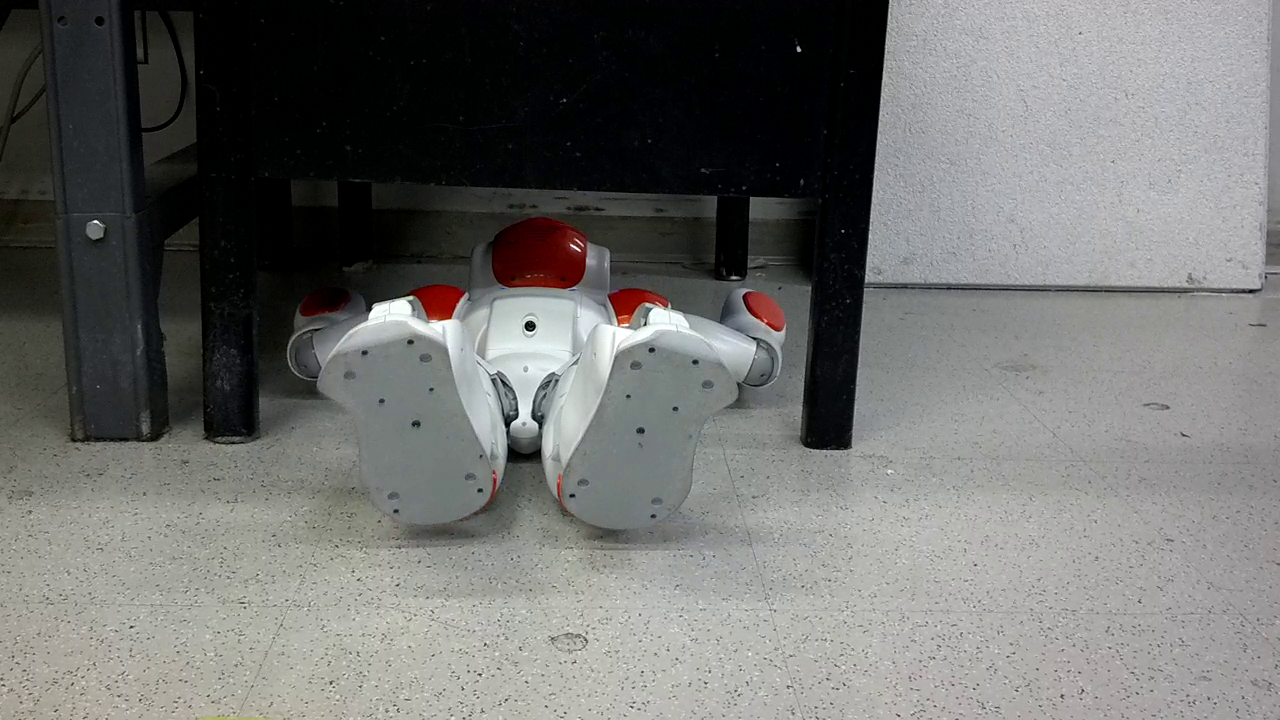
\includegraphics[width=0.25\textwidth]{crawl/under_table/20s.png}
  }
  \caption{Low-profile crawling gait for accessing vertically constrained spaces such as under a table.}
  \label{fig:nao_crawl1}
  \vspace*{-0.07in}
\end{figure}

Explain that this experiment is a demonstration of the gait being used to perform a task,
getting through a crawl space.

\begin{figure}
  \centerline{
    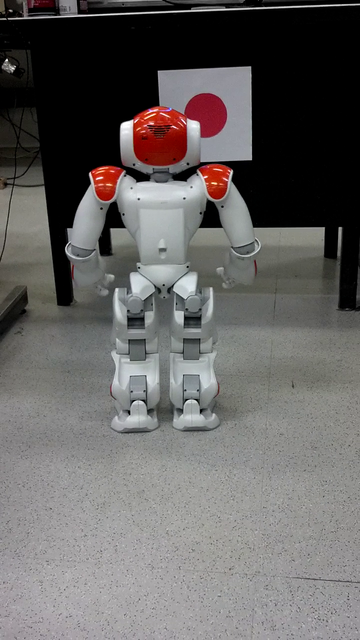
\includegraphics[width=0.2\textwidth]{crawl/walk_to/to/12s.png}
    \includegraphics[width=0.2\textwidth]{crawl/walk_to/to/18s.png}
    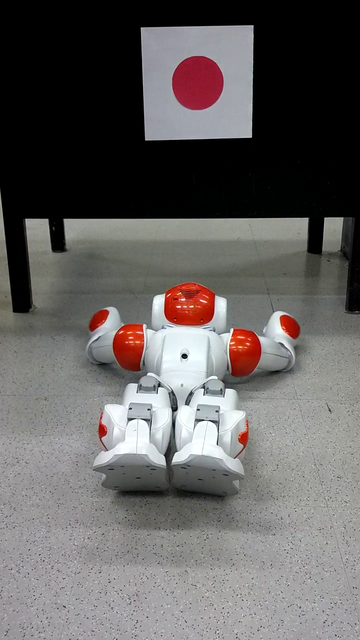
\includegraphics[width=0.2\textwidth]{crawl/walk_to/to/29s.png}
    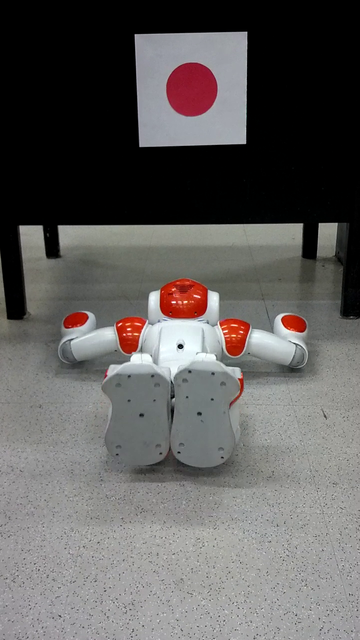
\includegraphics[width=0.2\textwidth]{crawl/walk_to/to/30s_2.png}
    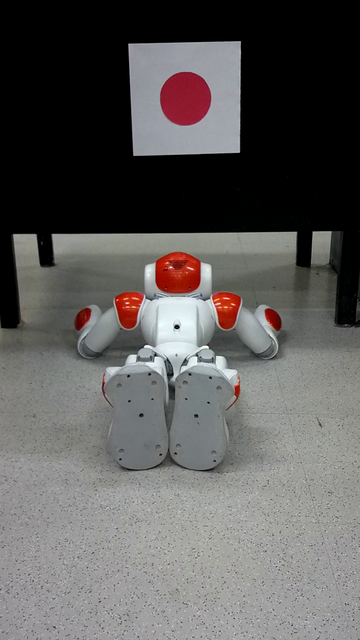
\includegraphics[width=0.2\textwidth]{crawl/walk_to/to/34s.png}
  }
  \vspace*{0.05in}
  \centerline{
    \includegraphics[width=0.2\textwidth]{crawl/walk_to/to/37s.png}
    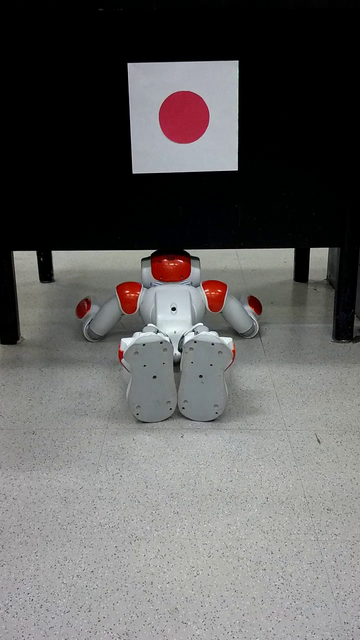
\includegraphics[width=0.2\textwidth]{crawl/walk_to/to/40s.png}
    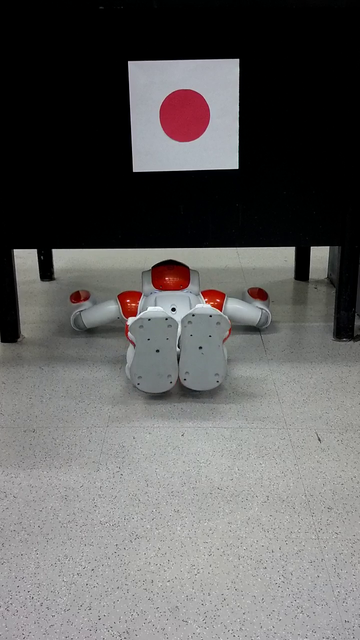
\includegraphics[width=0.2\textwidth]{crawl/walk_to/to/41s.png}
    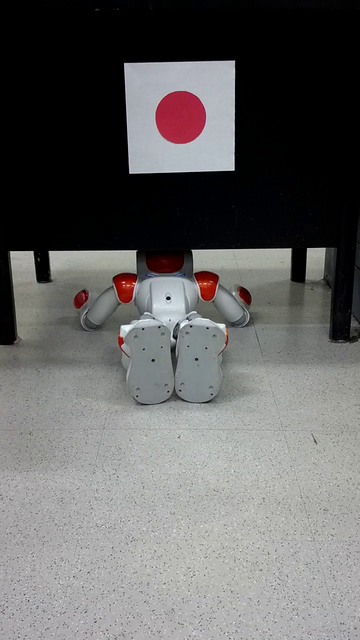
\includegraphics[width=0.2\textwidth]{crawl/walk_to/to/43s.png}
    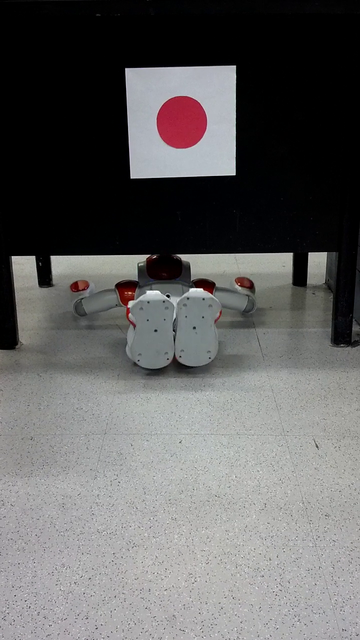
\includegraphics[width=0.2\textwidth]{crawl/walk_to/to/46s.png}
  }
  \vspace*{-0.05in}
  \caption{BLAH BLAH Approaching and crawling under an obstacle.
           A red dot is used as a marker for the direction in which the robot is commanded to move.
           When the robot approaches below a specified distance threshold from the obstacle,
           the crouch-down and crawl gait sequence is initiated.}
  \label{fig:nao_crawl3}
  \vspace*{-0.15in}
\end{figure}

\begin{figure}
  \centerline{
    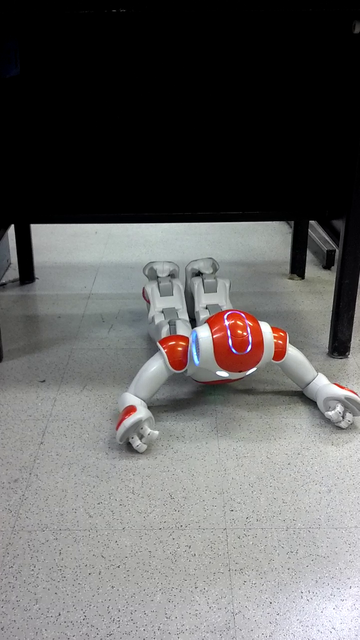
\includegraphics[width=0.2\textwidth]{crawl/walk_to/from/8s.png}
    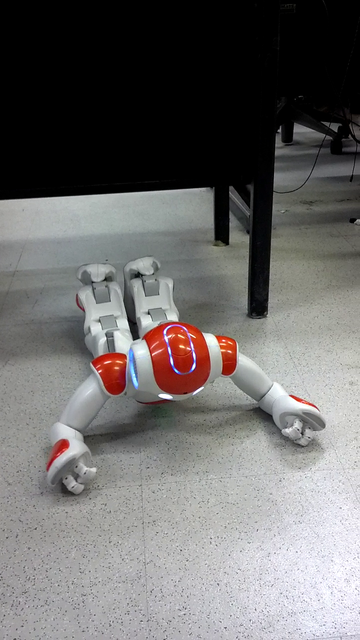
\includegraphics[width=0.2\textwidth]{crawl/walk_to/from/15s.png}
    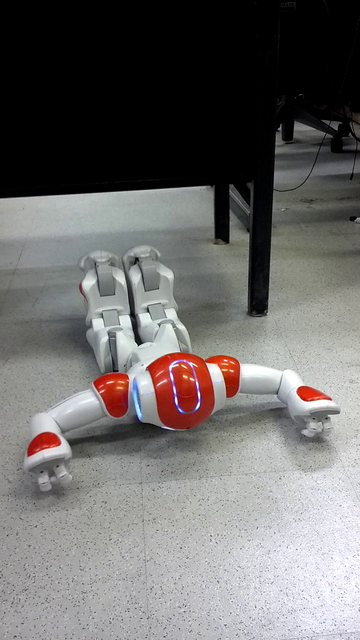
\includegraphics[width=0.2\textwidth]{crawl/walk_to/from/16s.png}
    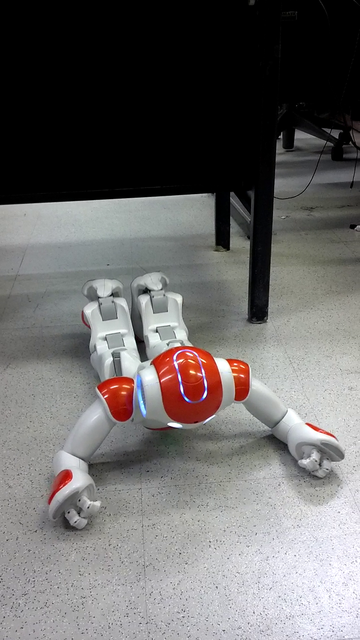
\includegraphics[width=0.2\textwidth]{crawl/walk_to/from/17s.png}
    \includegraphics[width=0.2\textwidth]{crawl/walk_to/from/18s.png}
  }
  \vspace*{0.05in}
  \centerline{
    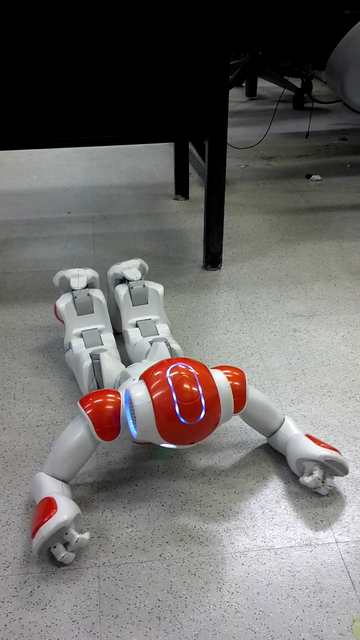
\includegraphics[width=0.2\textwidth]{crawl/walk_to/from/24s.png}
    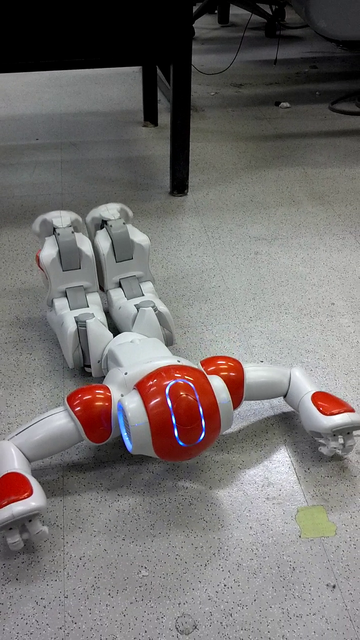
\includegraphics[width=0.2\textwidth]{crawl/walk_to/from/30s.png}
    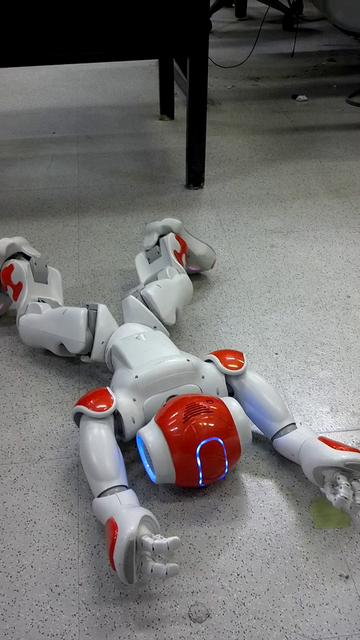
\includegraphics[width=0.2\textwidth]{crawl/walk_to/from/32s.png}
    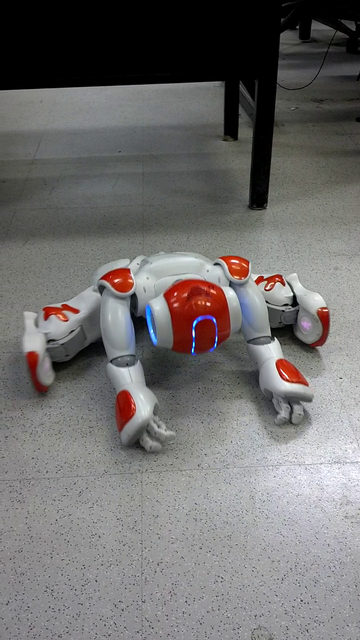
\includegraphics[width=0.2\textwidth]{crawl/walk_to/from/35s.png}
    \includegraphics[width=0.2\textwidth]{crawl/walk_to/from/37s.png}
  }
  \vspace*{-0.05in}
  \caption{BLAH BLAH Crawling under an obstacle and transitioning back to stand posture.}
  \label{fig:nao_crawl4}
  \vspace*{-0.01in}
  \vspace*{-0.05in}
\end{figure}

Here is a plot of the joint angles of the gait, showing its periodicity.

\begin{figure}
  \centerline{
    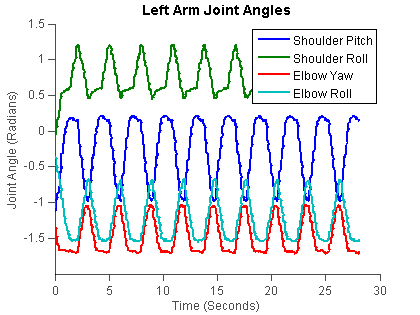
\includegraphics[width=0.5\textwidth]{crawl/joint_angles/LeftArmJointAngles.png}
    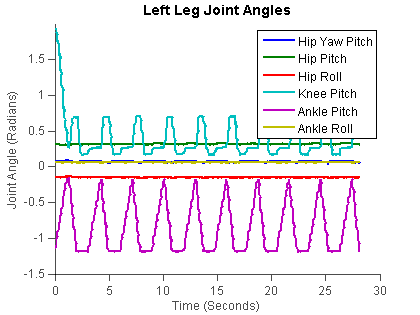
\includegraphics[width=0.5\textwidth]{crawl/joint_angles/LeftLegJointAngles.png}
  }
  \vspace*{-0.05in}
  \caption{Measured motor joint angles during multiple iterations of the periodic crawling gait.
           While the crawling gait is laterally symmetric, the asymmetry in measured angles is due to the
           definitions of the robot frame and joint frame in the NAO API, which essentially forms a mirror
           asymmetry between the left and right joints.}
  \label{fig:nao_joint_angles1}
  \vspace*{-0.1in}
\end{figure}

This is a full plot of the entire sequence, from walking, to crawling, to walking.

\begin{figure}
  \centerline{
    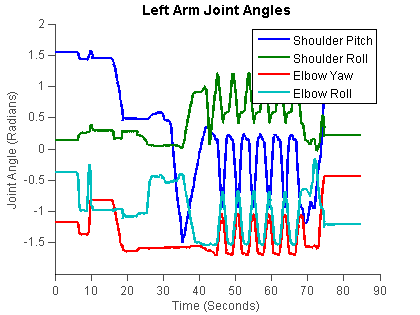
\includegraphics[width=0.5\textwidth]{crawl/joint_angles_long_sequence/LeftArmJointAngles_longSequence.png}
    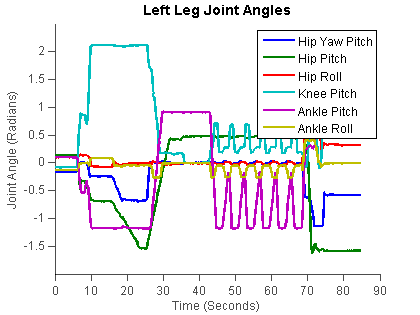
\includegraphics[width=0.5\textwidth]{crawl/joint_angles_long_sequence/LeftLegJointAngles_longSequence.png}
  }
  \vspace*{-0.05in}
  \caption{Measured joint angles for a sequence of transitioning from standing to crouch to crawling,
           crawling under a table, and then returning to crouch.}
  \label{fig:nao_joint_angles_long_seq}
  \vspace*{-0.2in}
\end{figure}

This plot shows the current draws of the arm and leg joints.
There are some distinct patterns, but is hard to relate torques directly.

\begin{figure}
  \centerline{
    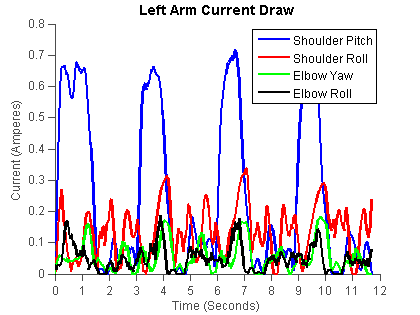
\includegraphics[width=0.5\textwidth]{crawl/current_draws/LeftArmCurrentDraw.png}
    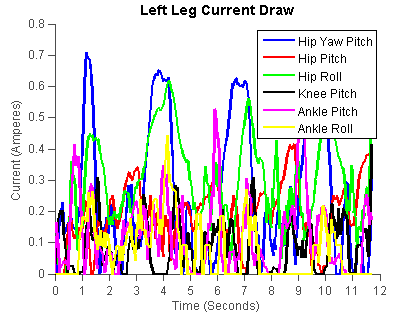
\includegraphics[width=0.5\textwidth]{crawl/current_draws/LeftLegCurrentDraw.png}
  }
  \vspace*{-0.03in}
  \caption{Measured motor current draws during multiple iterations of the periodic crawling gait.}
  \label{fig:nao_currents}
  \vspace*{-0.23in}
\end{figure}


THROW IN A V-REP PICTURE OR 4.


WHAT WERE THE TRIPLET PARAMETERS?

Insert plot of the optimization process.

PUT IN HOW MANY ITERATIONS IT TOOK TO FINISH.
PUT IN HOW MANY ITERATIONS IT TOOK TO KINDA CONVERGE.
THROW IN THE OTHER RELEVANT STATISTICS LIKE NUMBER OF CHILDREN ETC.

These plots show the theoretical optimization costs of the nominal and optimized
triplet parameters. 

\begin{figure}
  \vspace*{-0.12in}
  \centerline{
    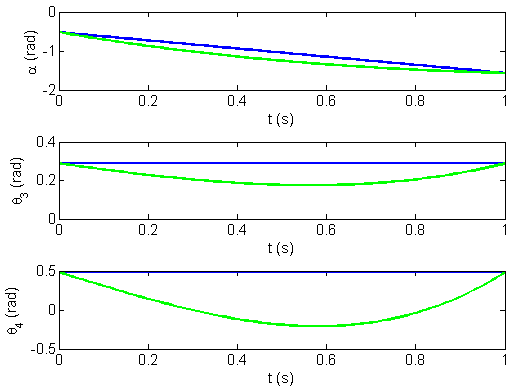
\includegraphics[width=0.75\textwidth]{crawl/cost/ga_cost2_plot1_edit1.png}
  }
  \vspace*{-0.15in}
  \caption{Optimization of crawling motion. Blue lines: nominal time trajectories of the angle triplet 
           $(\alpha,\theta_3,\theta_4)$; Green lines: optimized time trajectories. }
  \vspace*{-0.17in}
  \label{fig:optimal}
\end{figure}

Ok, so now, how does it do with these new optimizations?
We use the V-REP here instead of the currents from the robot because they are easier to interpret.

Insert pictures of the Projected Profile optimized gait.

Insert pictures of the V-REP gaits overlaid onto the
optimized gait.

Insert pictures of the torque graphs for the nominal and optimized gaits.

\begin{figure}
  \centerline{
    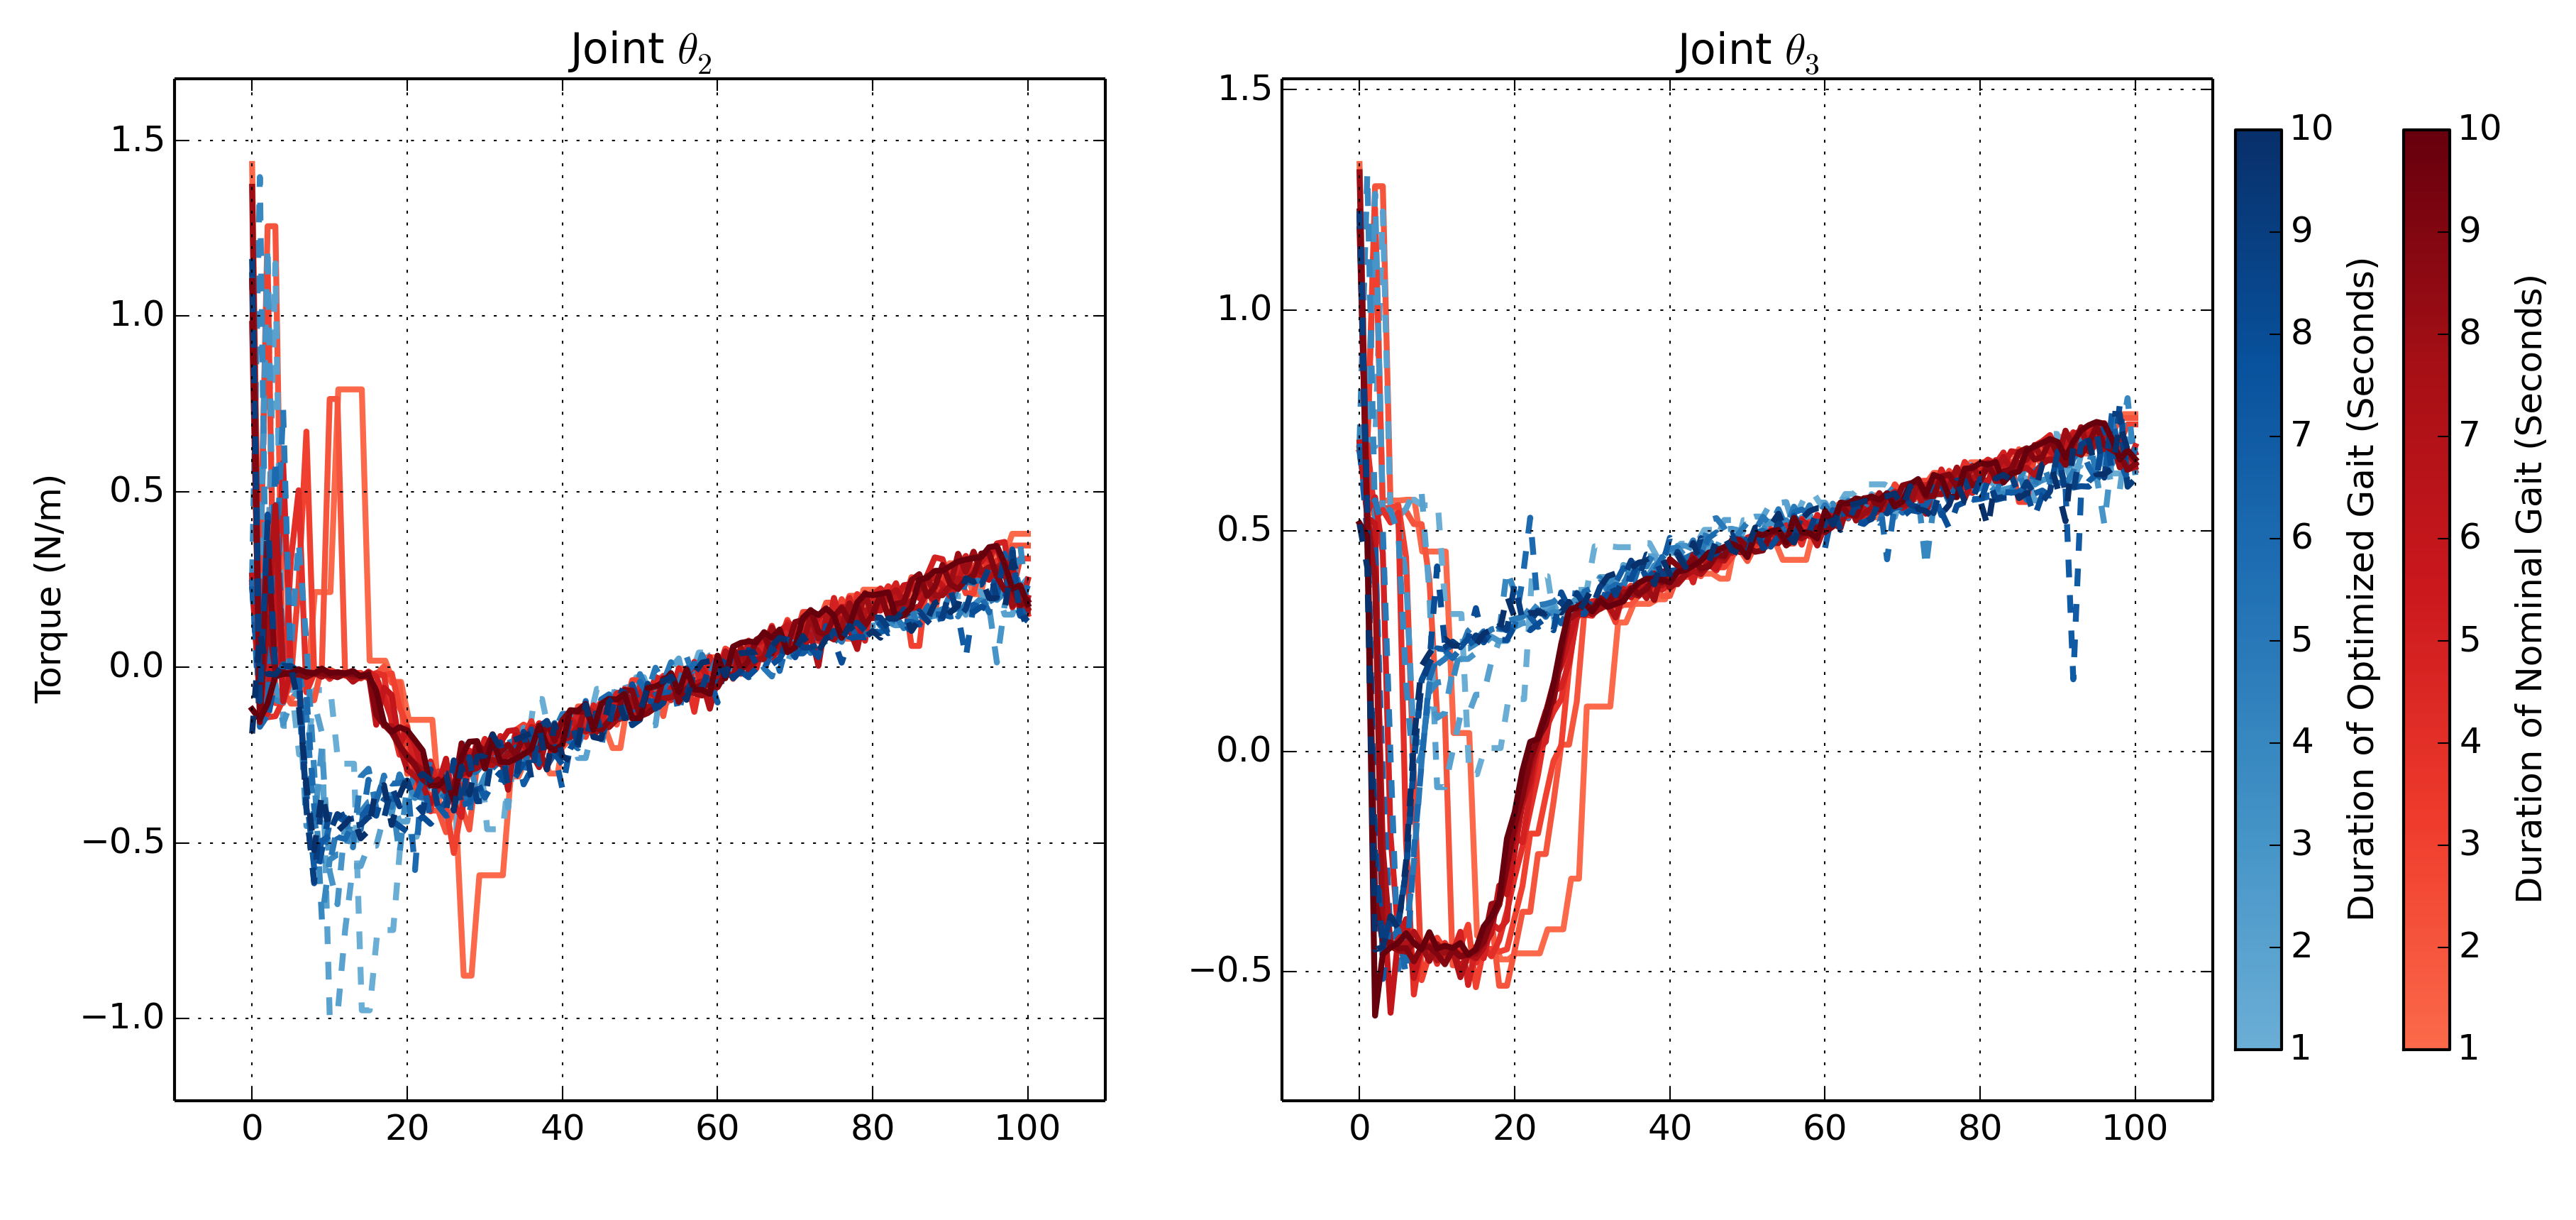
\includegraphics[width=\textwidth]{crawl/torques/trimmed/joint2_3_torques.png}
  }
  % \vspace*{0.05in}
  \centerline{
    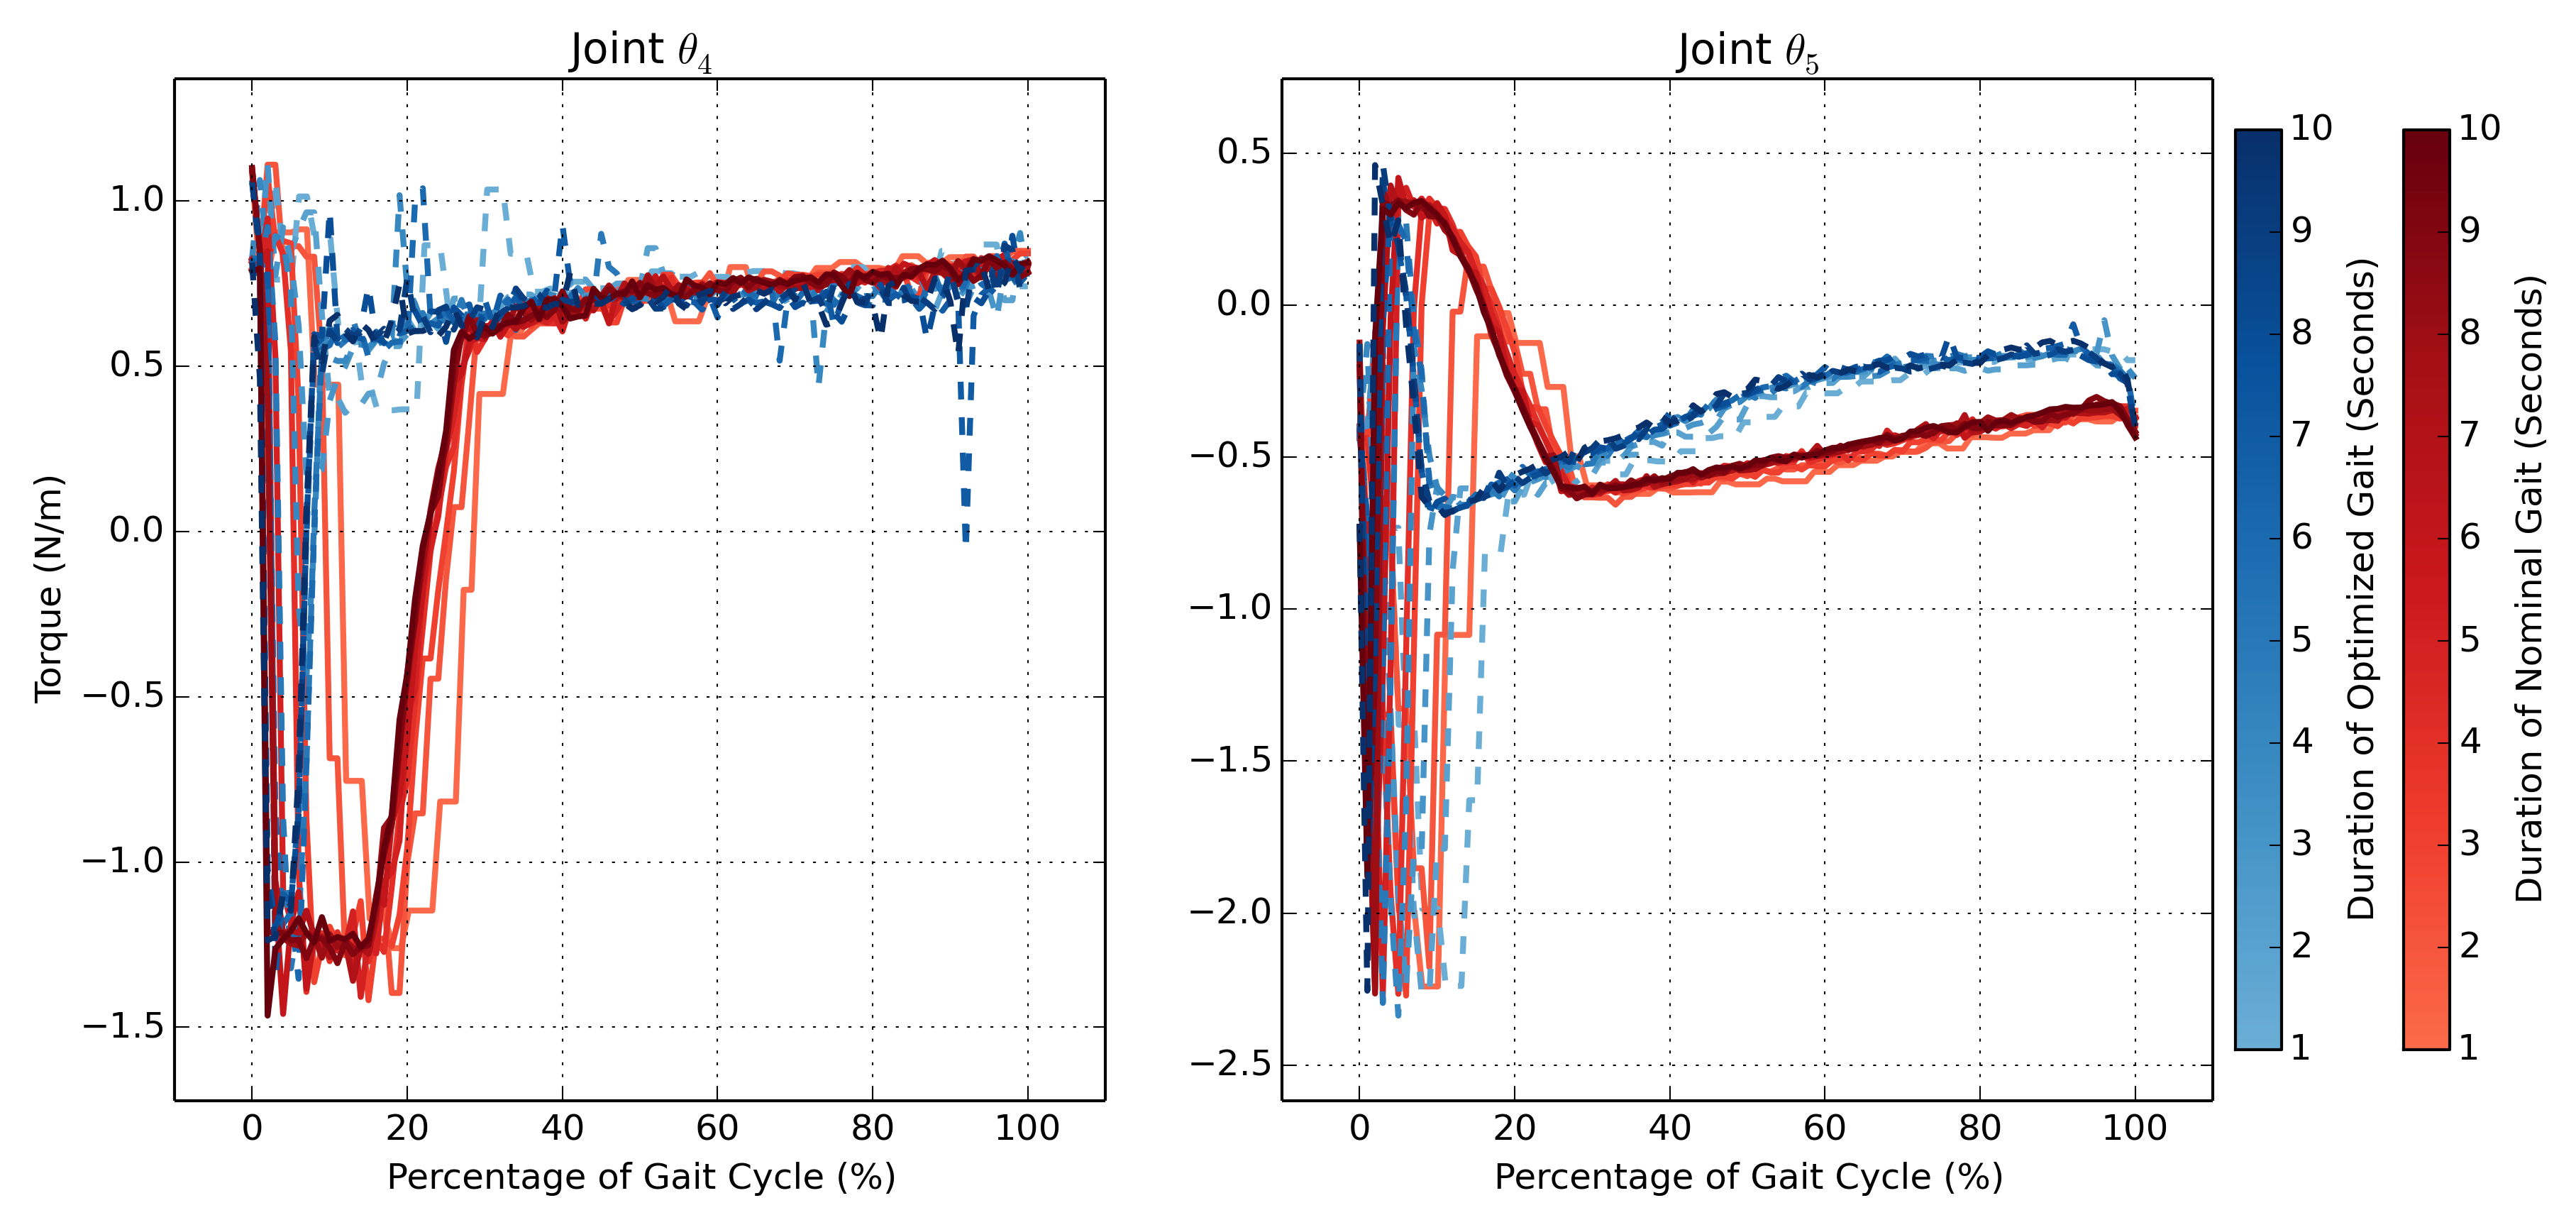
\includegraphics[width=\textwidth]{crawl/torques/trimmed/joint4_5_torques.png}
  }
  % \vspace*{-0.05in}
  \caption{BLAH BLAH Simulated joint torques for the different times. Nominal and optimized.}
  \label{fig:vrep_joint_torques_by_joint1}
  % \vspace*{-0.01in}
  % \vspace*{-0.05in}
\end{figure}

\begin{figure}
  \centerline{
    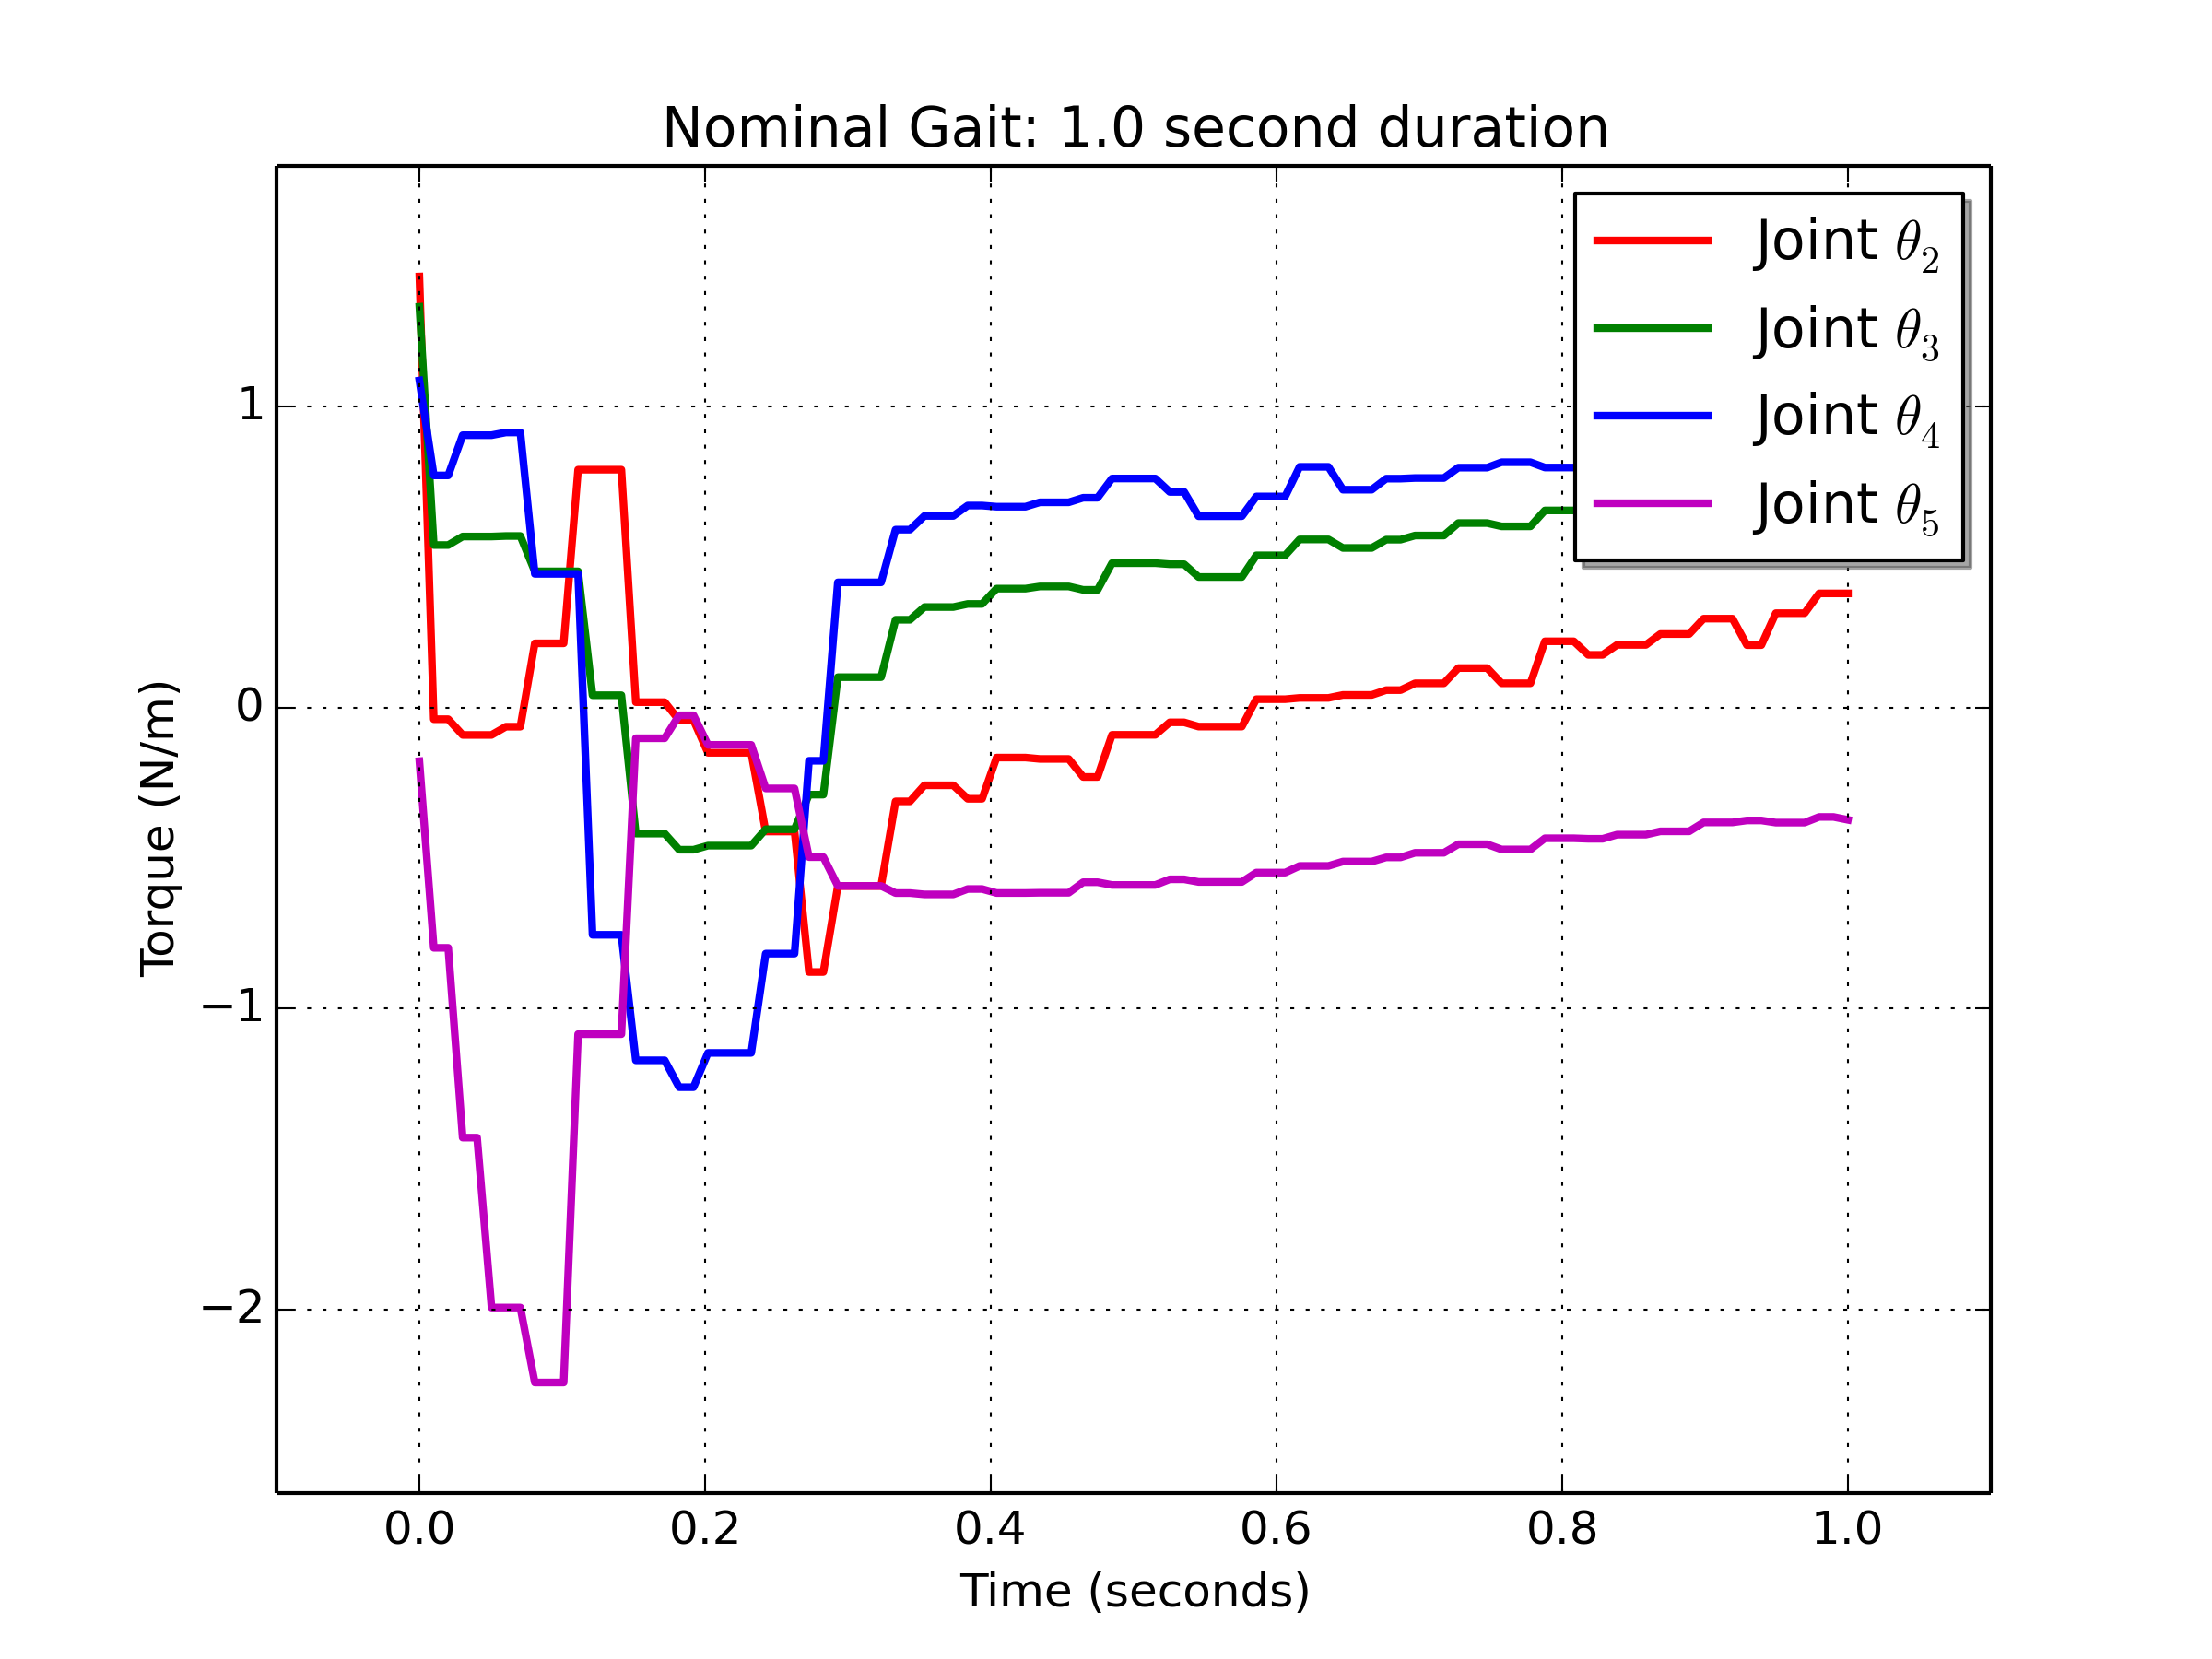
\includegraphics[width=0.5\textwidth]{crawl/torques/nom_torques_duration_1.0_1.png}
    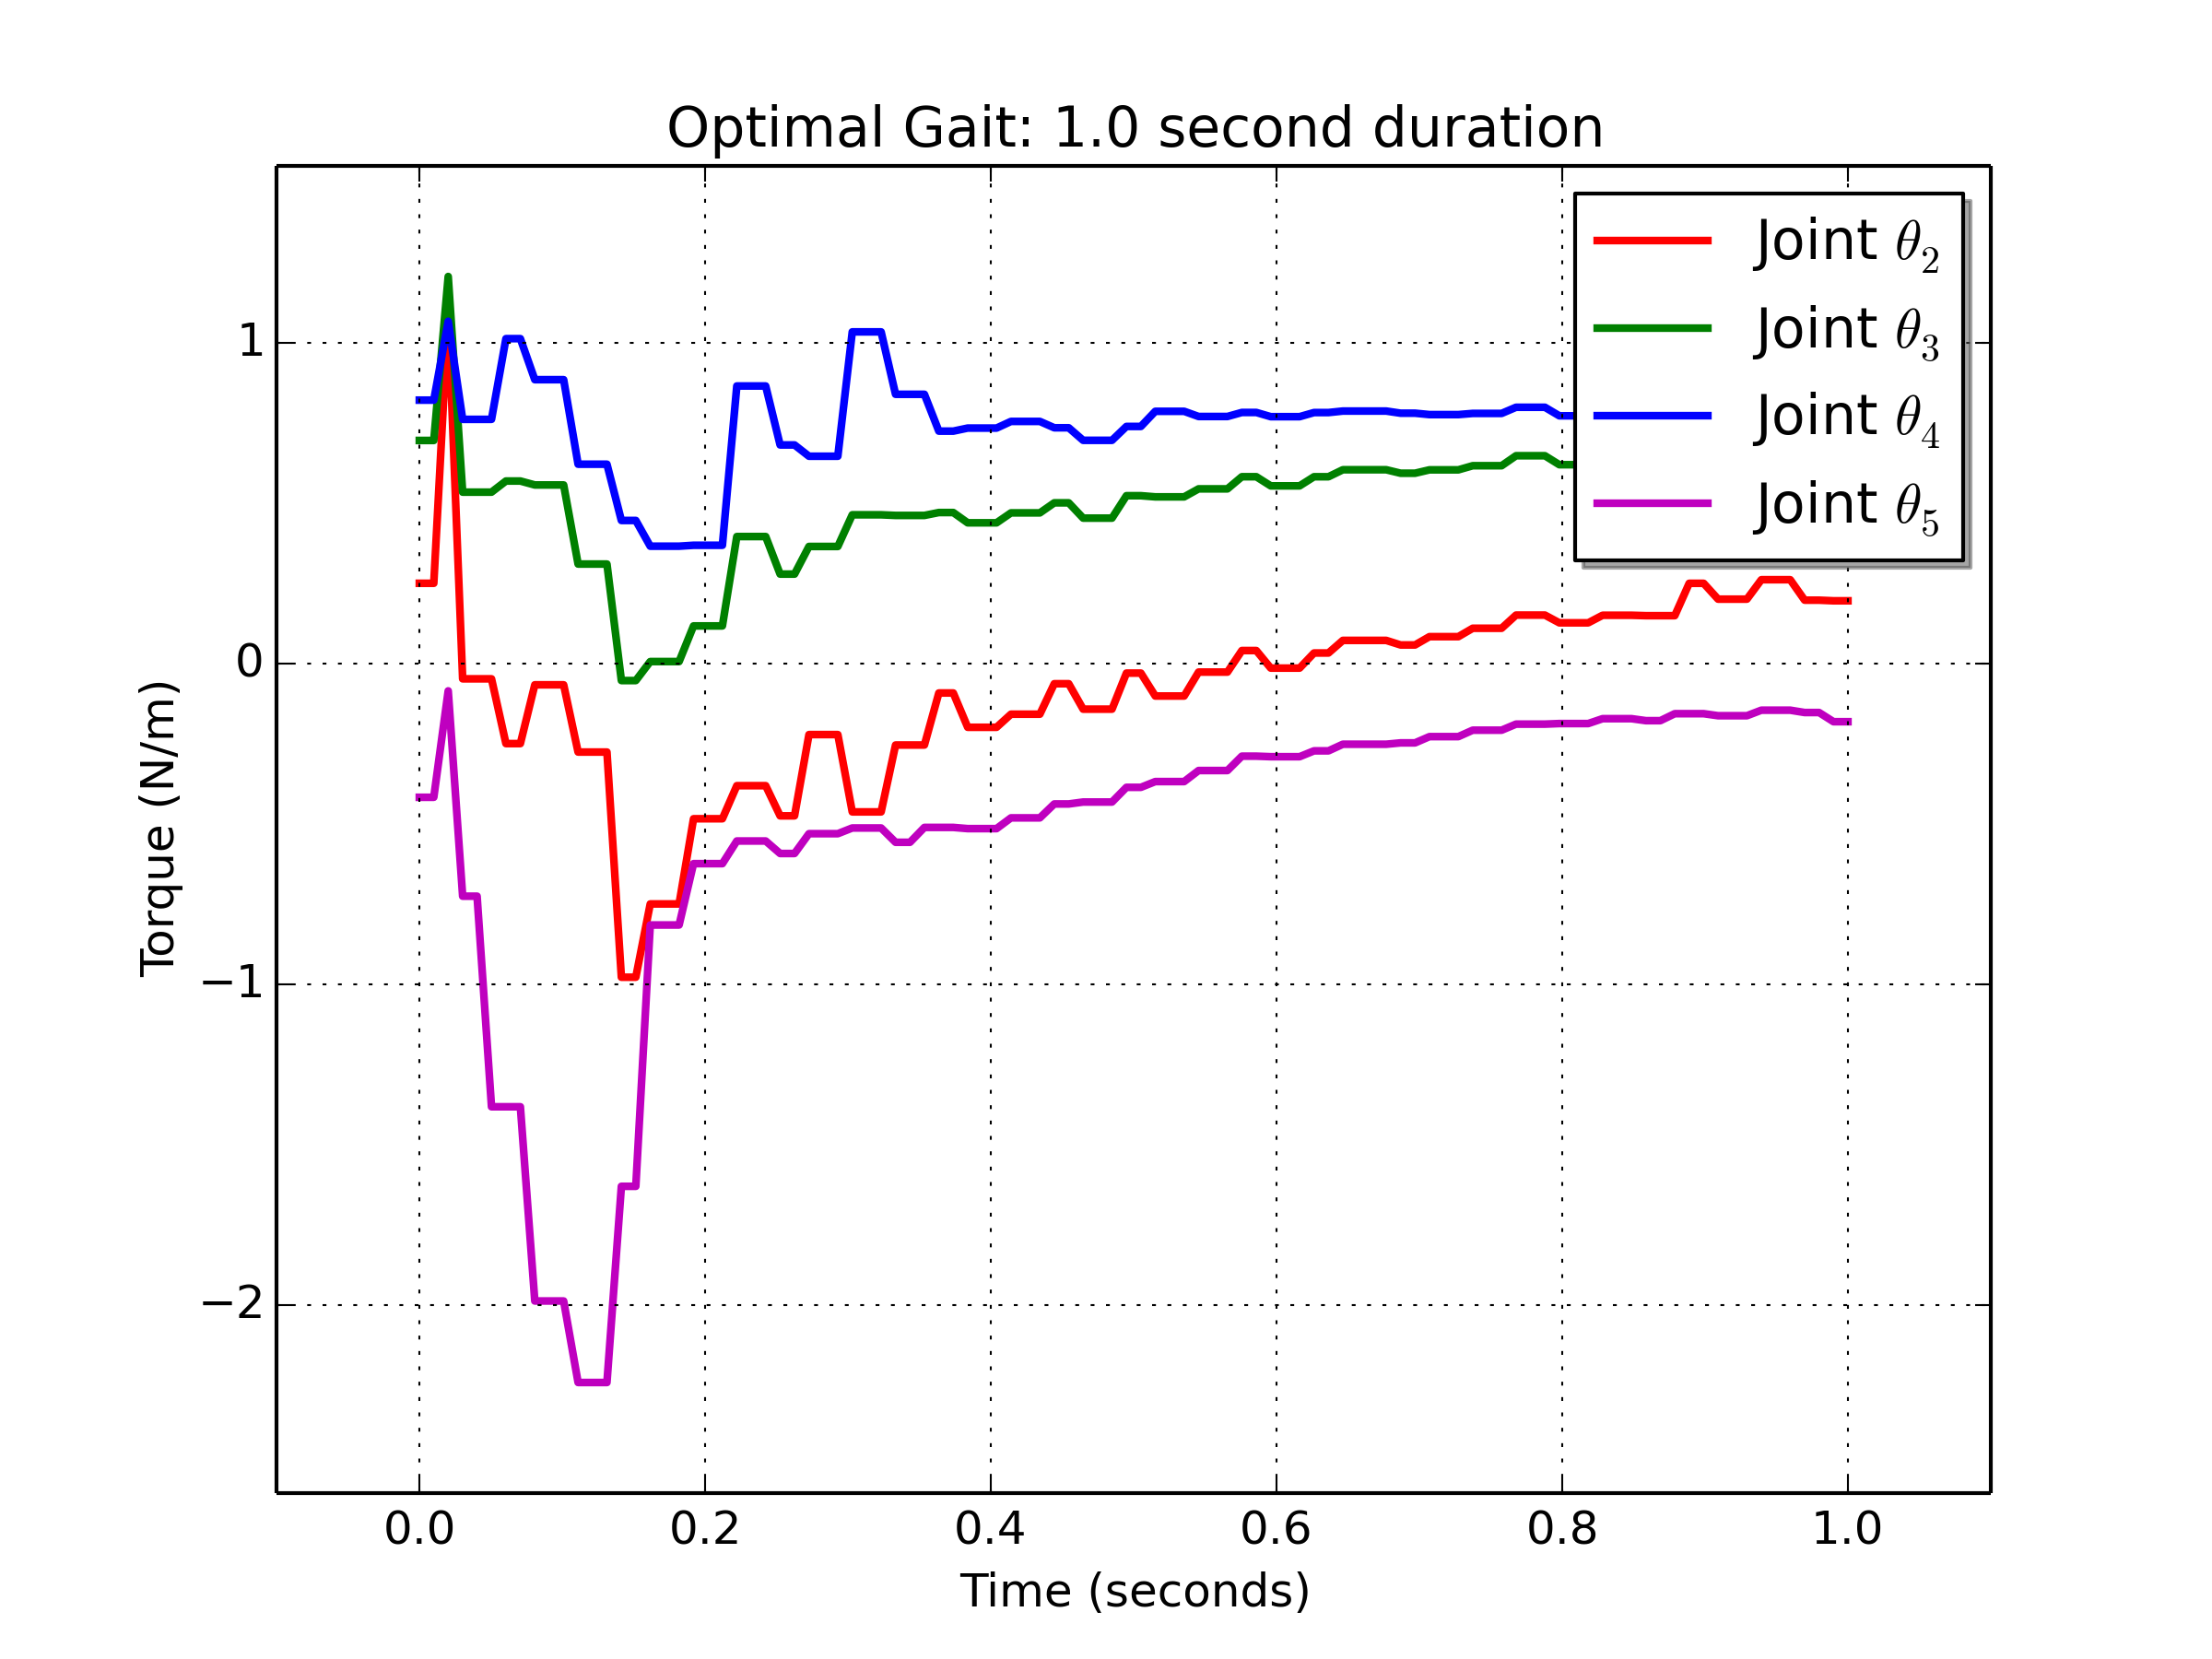
\includegraphics[width=0.5\textwidth]{crawl/torques/opt_torques_duration_1.0_1.png}
  }
  \vspace*{0.05in}
  \centerline{
    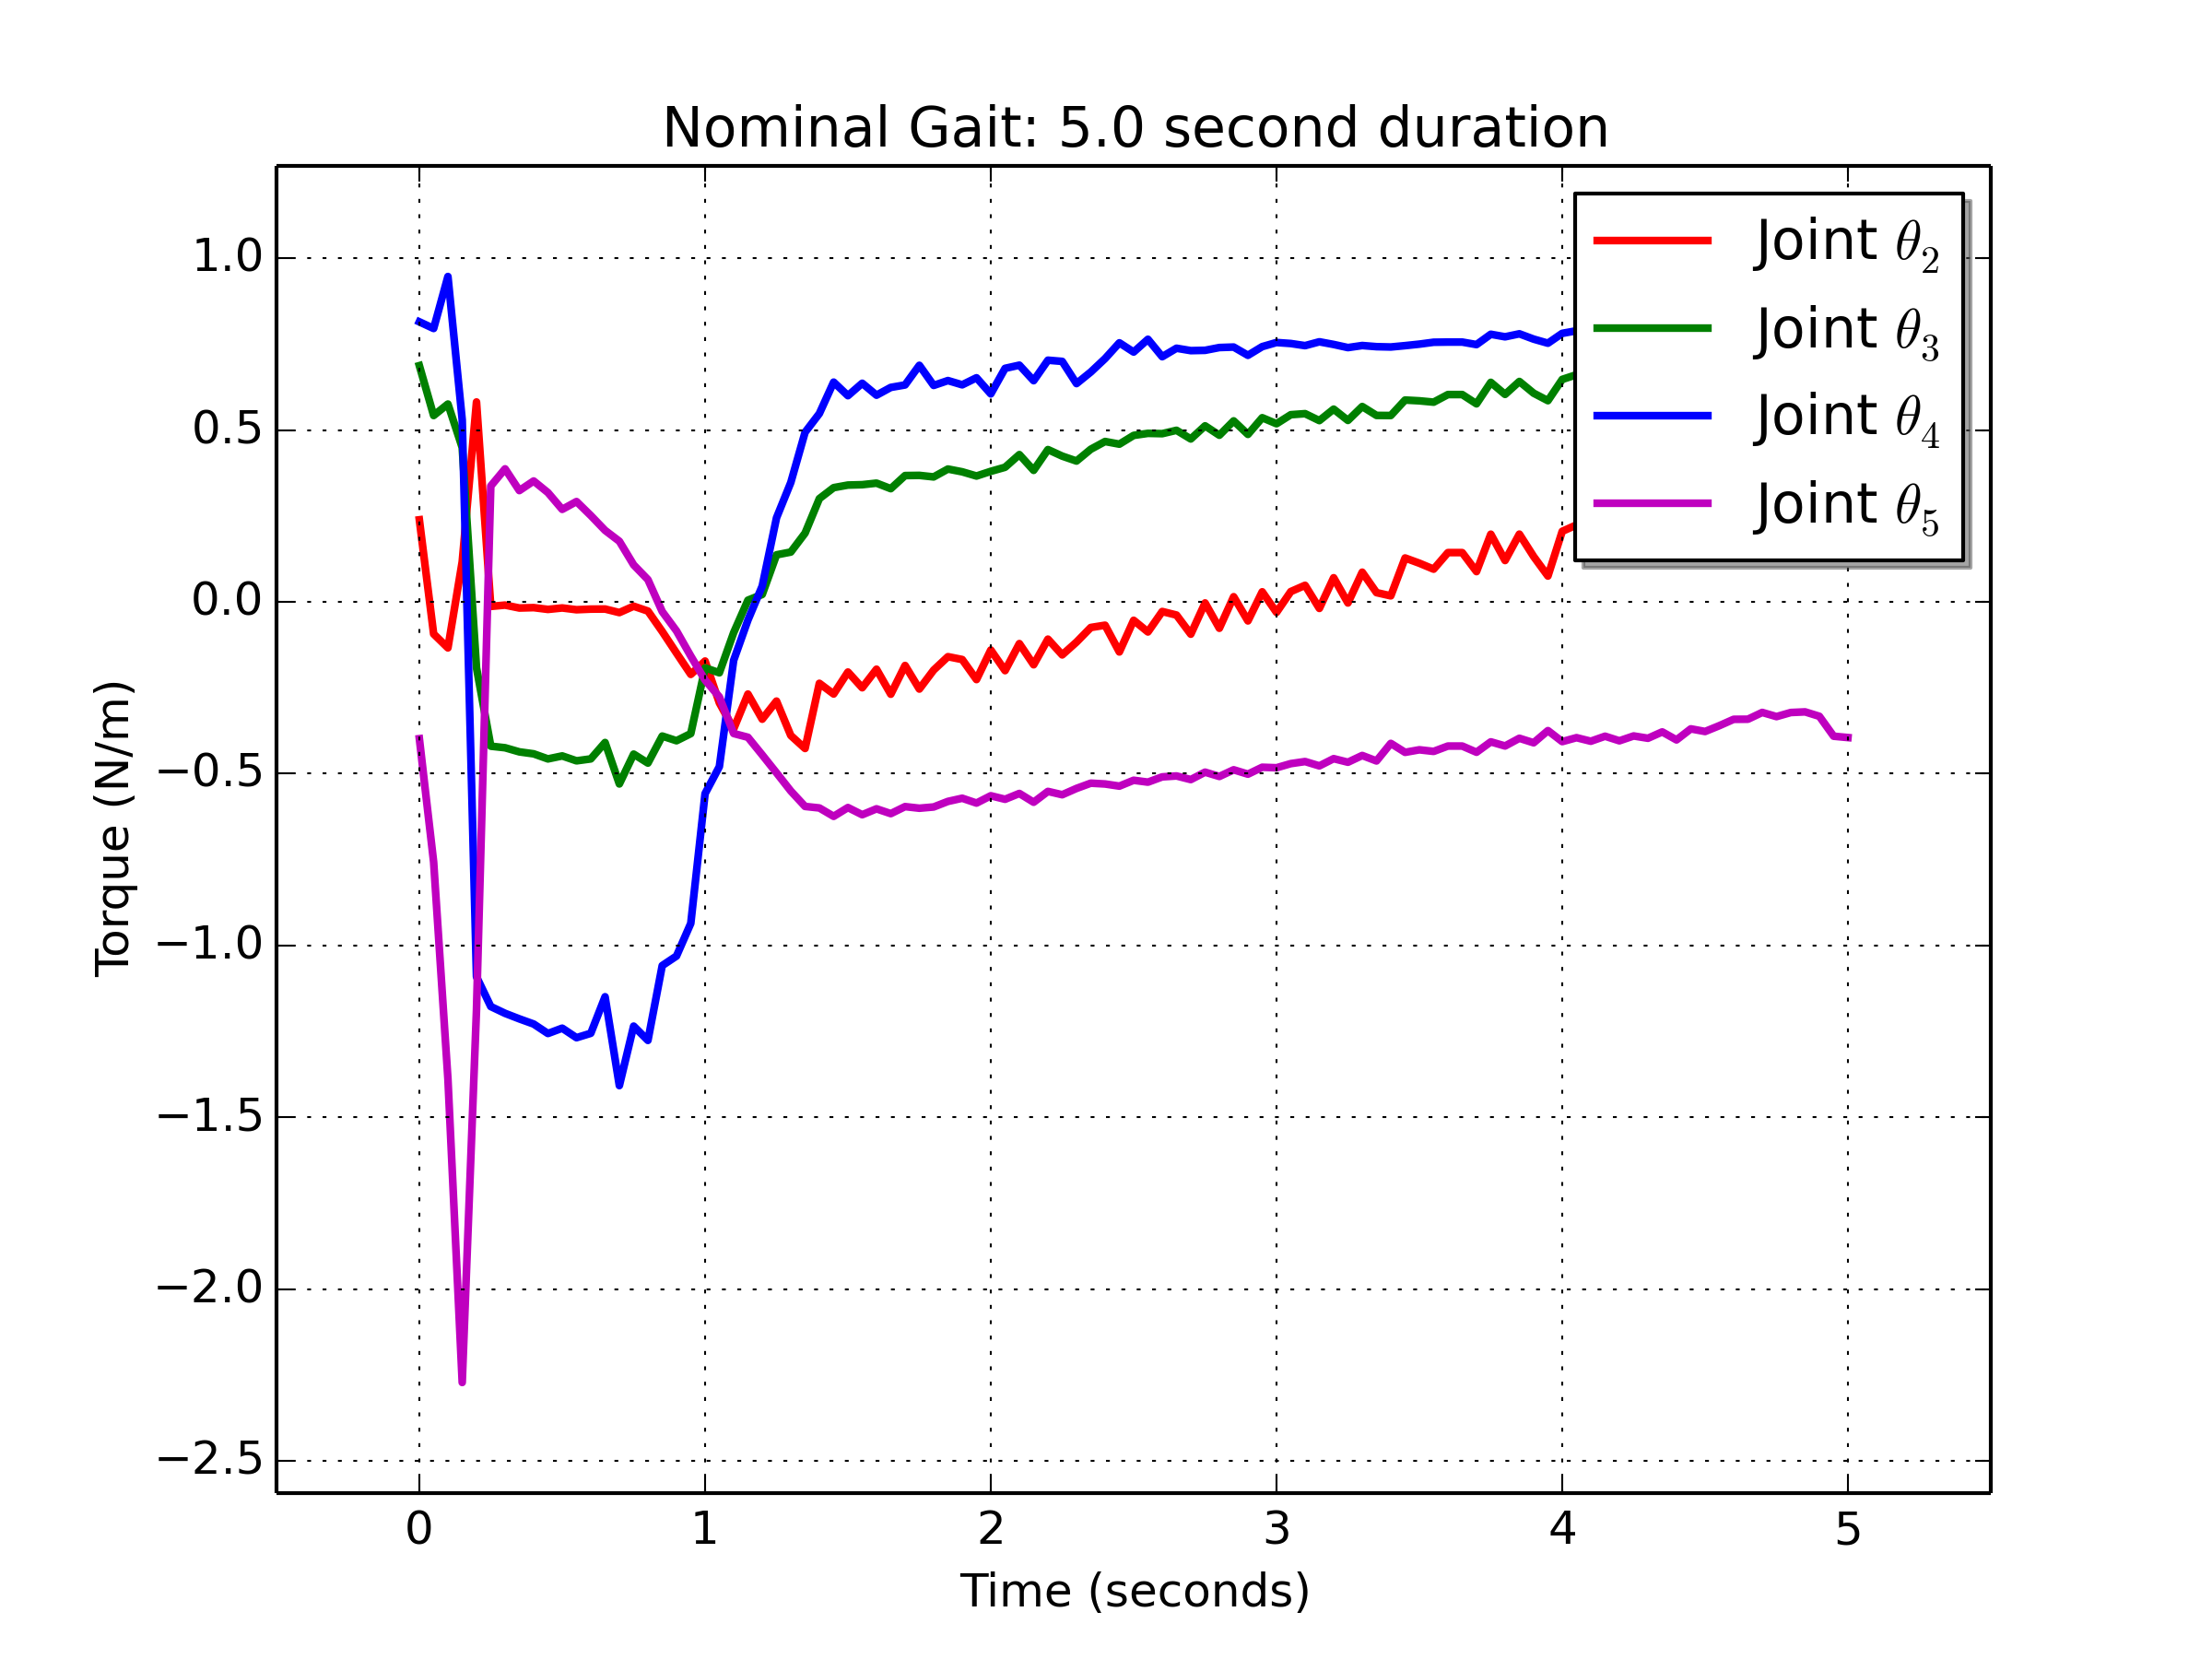
\includegraphics[width=0.5\textwidth]{crawl/torques/nom_torques_duration_5.0_1.png}
    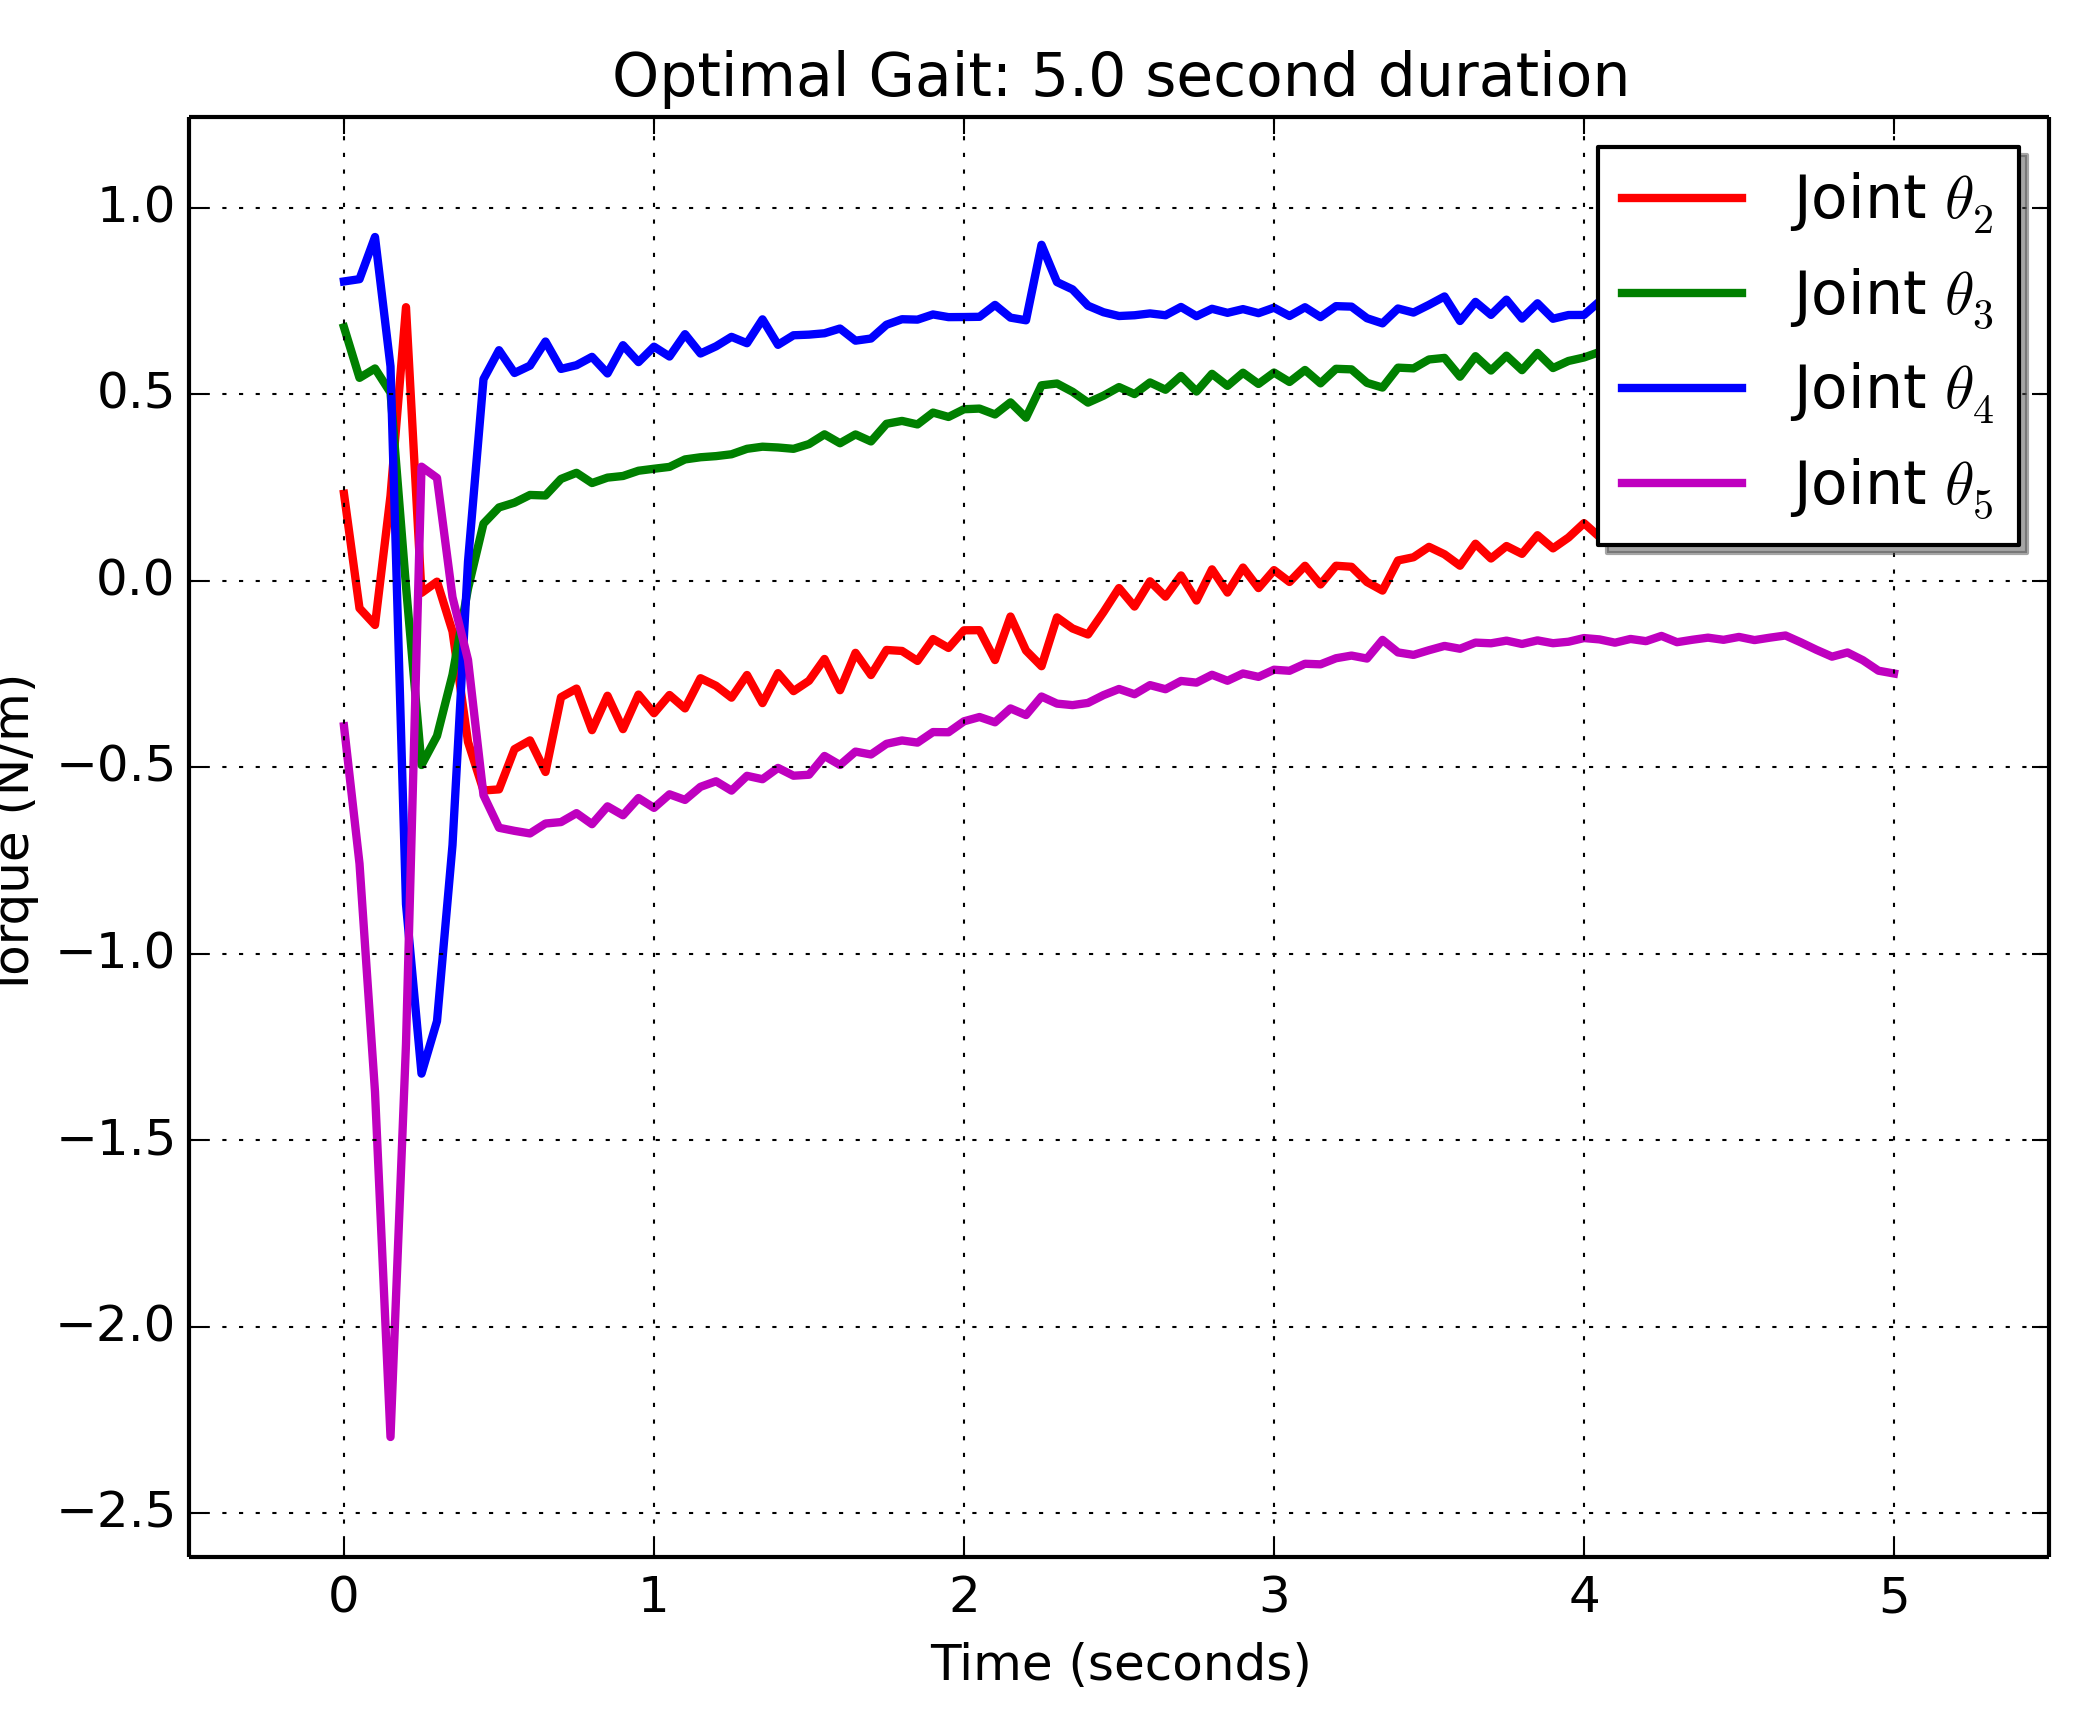
\includegraphics[width=0.5\textwidth]{crawl/torques/opt_torques_duration_5.0_1.png}
  }
  \vspace*{0.05in}
  \centerline{
    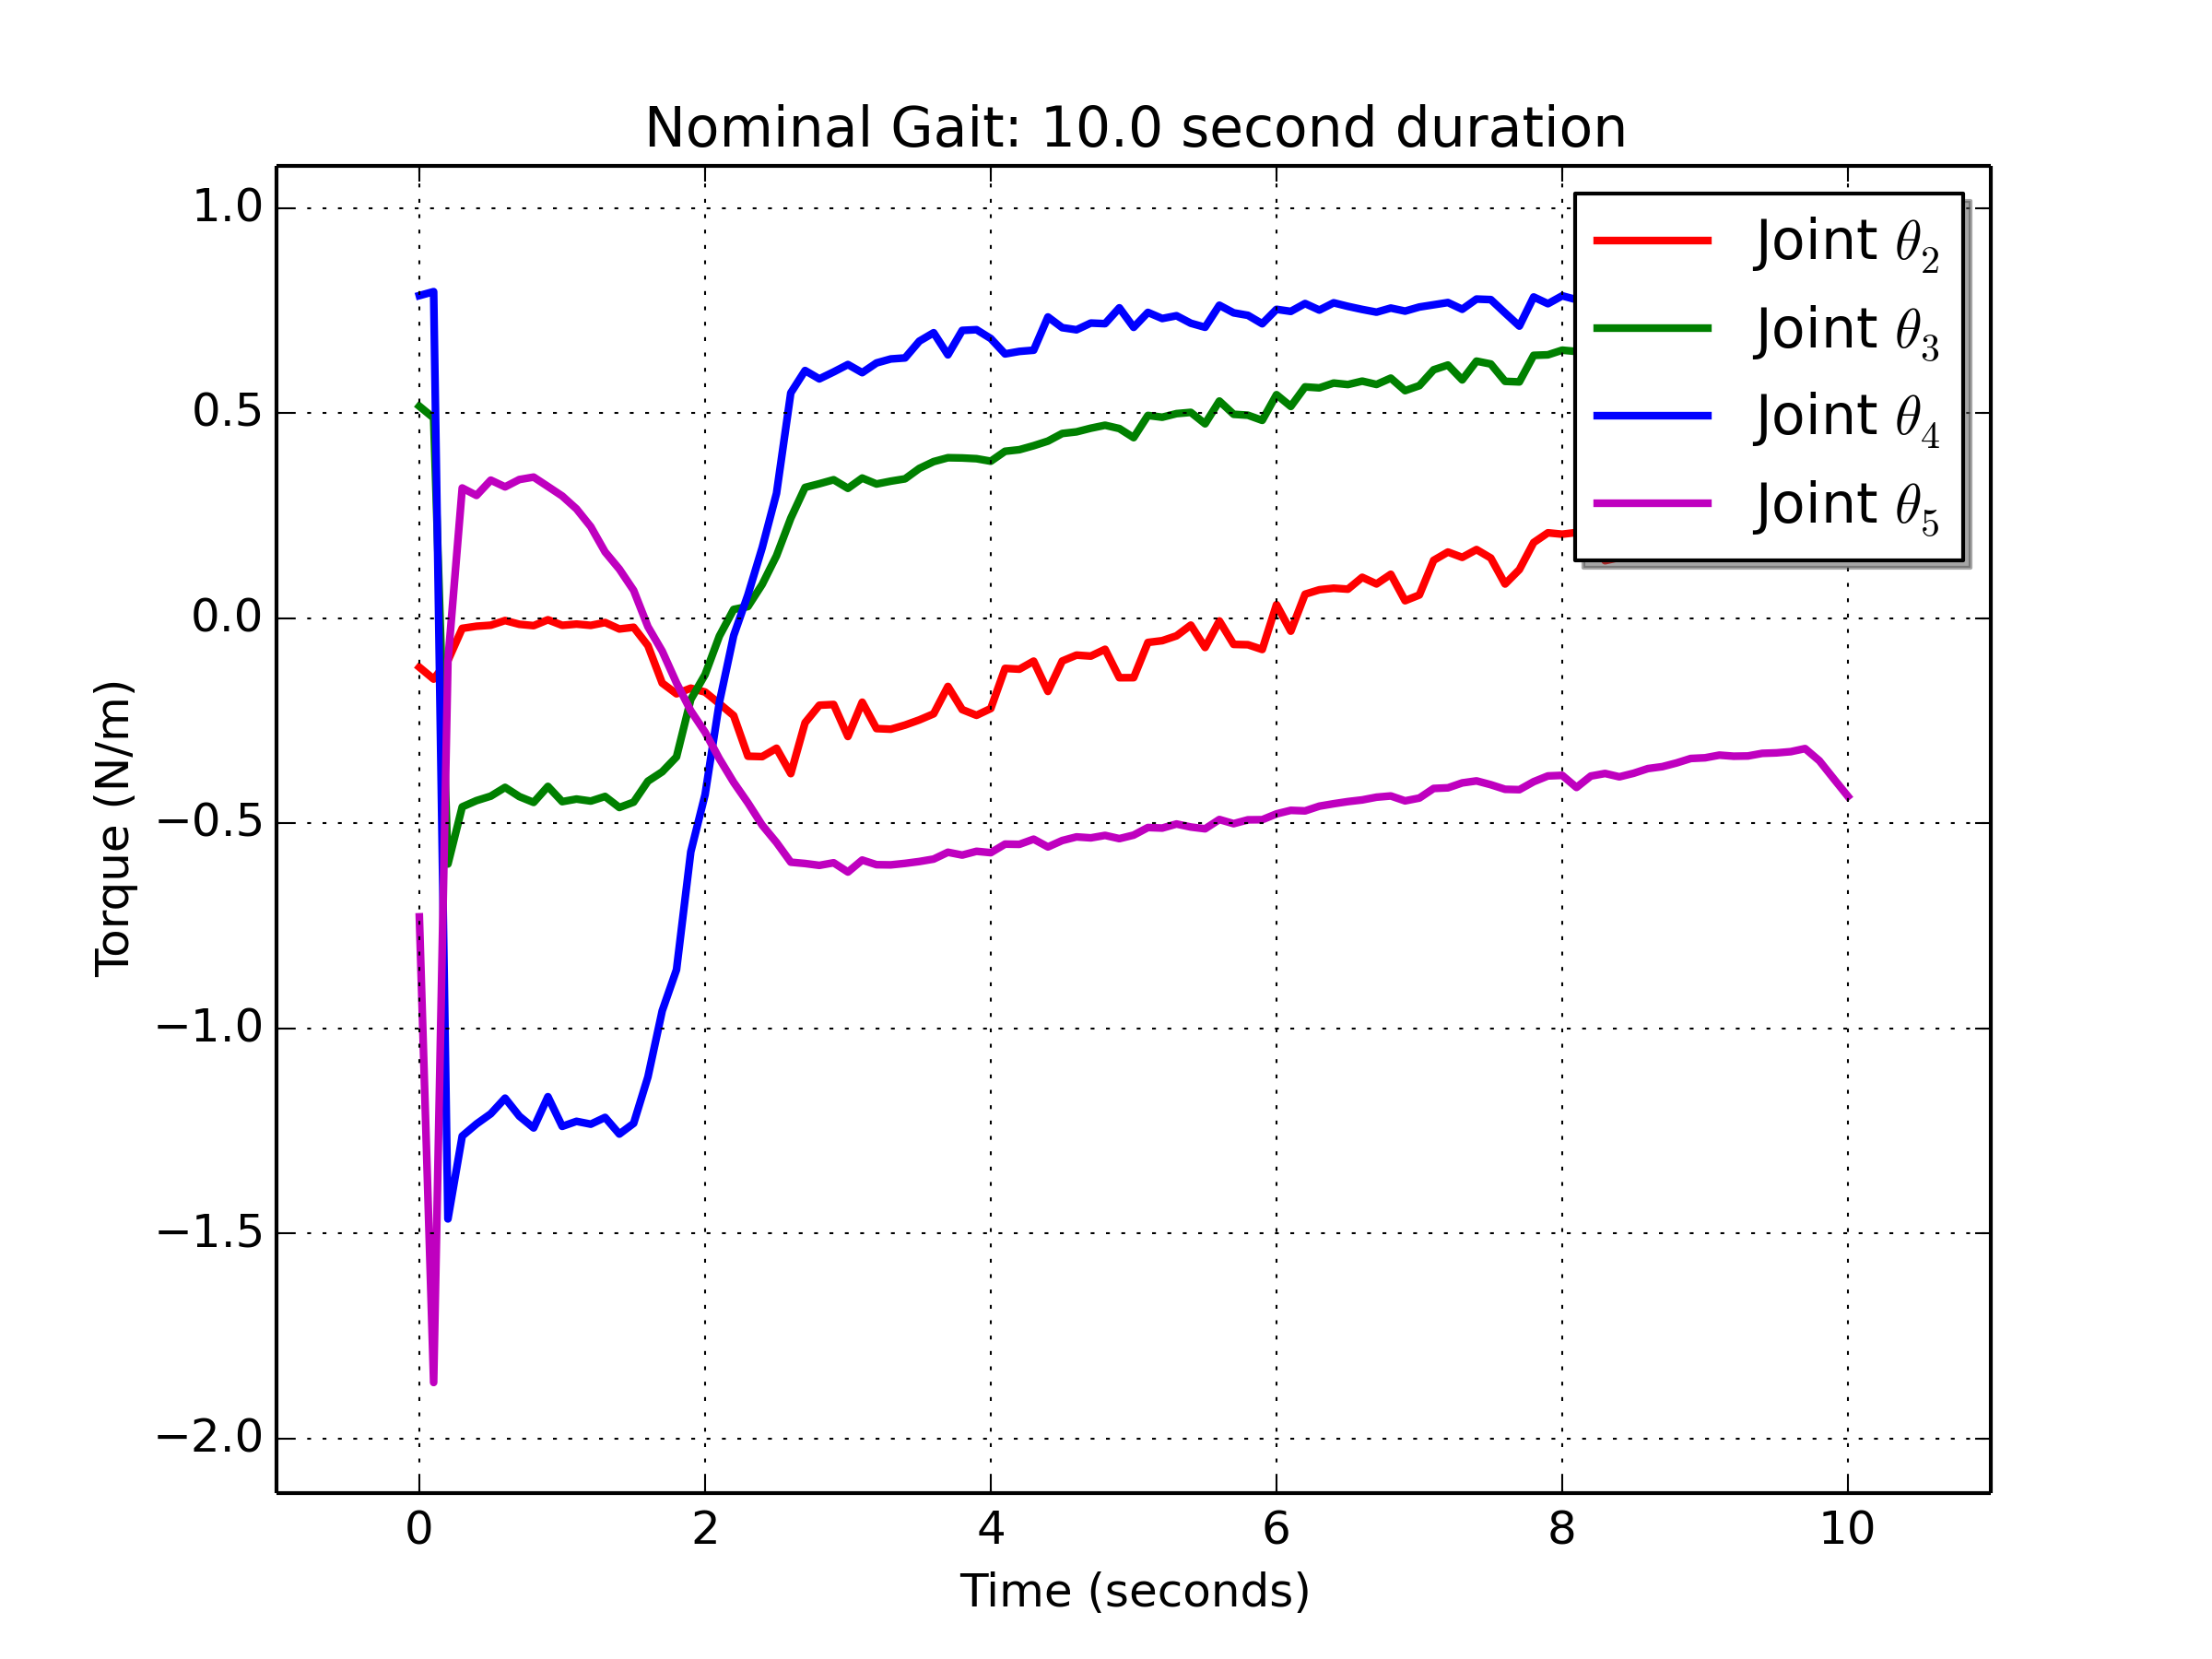
\includegraphics[width=0.5\textwidth]{crawl/torques/nom_torques_duration_10.0_1.png}
    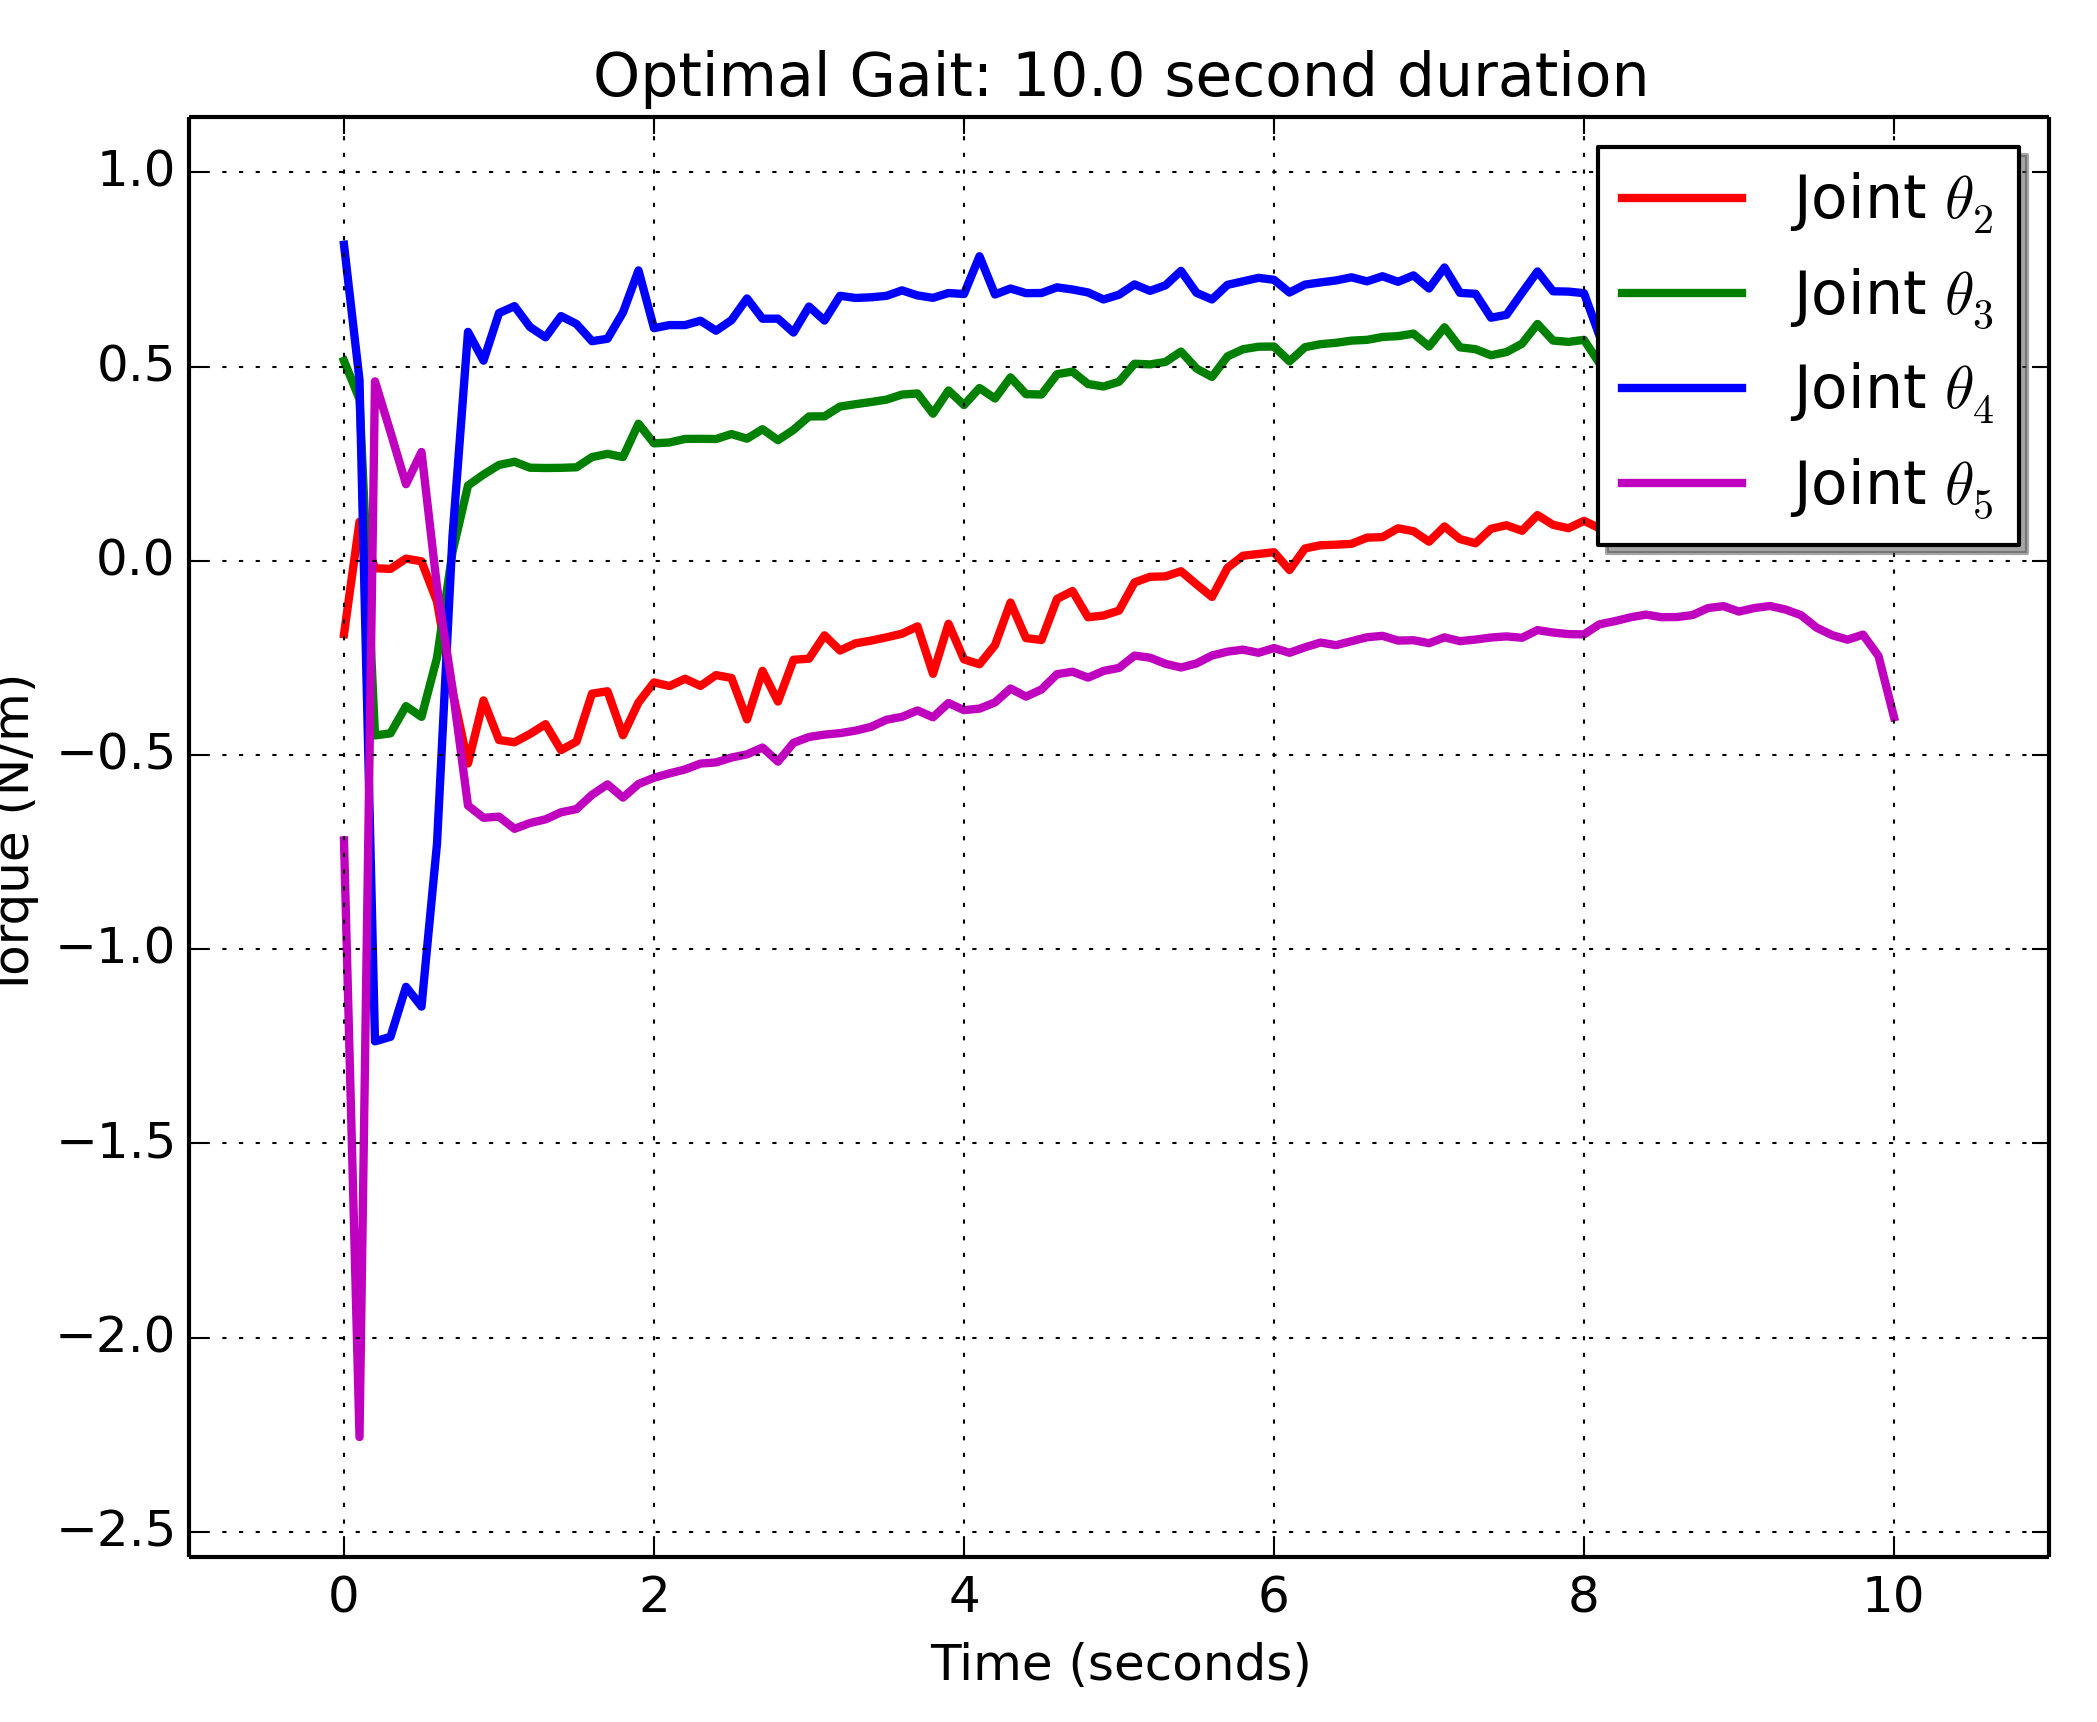
\includegraphics[width=0.5\textwidth]{crawl/torques/opt_torques_duration_10.0_1.png}
  }
  \vspace*{-0.05in}
  \caption{BLAH BLAH Simulated joint torques for the different times. Nominal and optimized.}
  \label{fig:vrep_joint_torques_by_duration1}
  \vspace*{-0.01in}
  \vspace*{-0.05in}
\end{figure}

\begin{figure}
  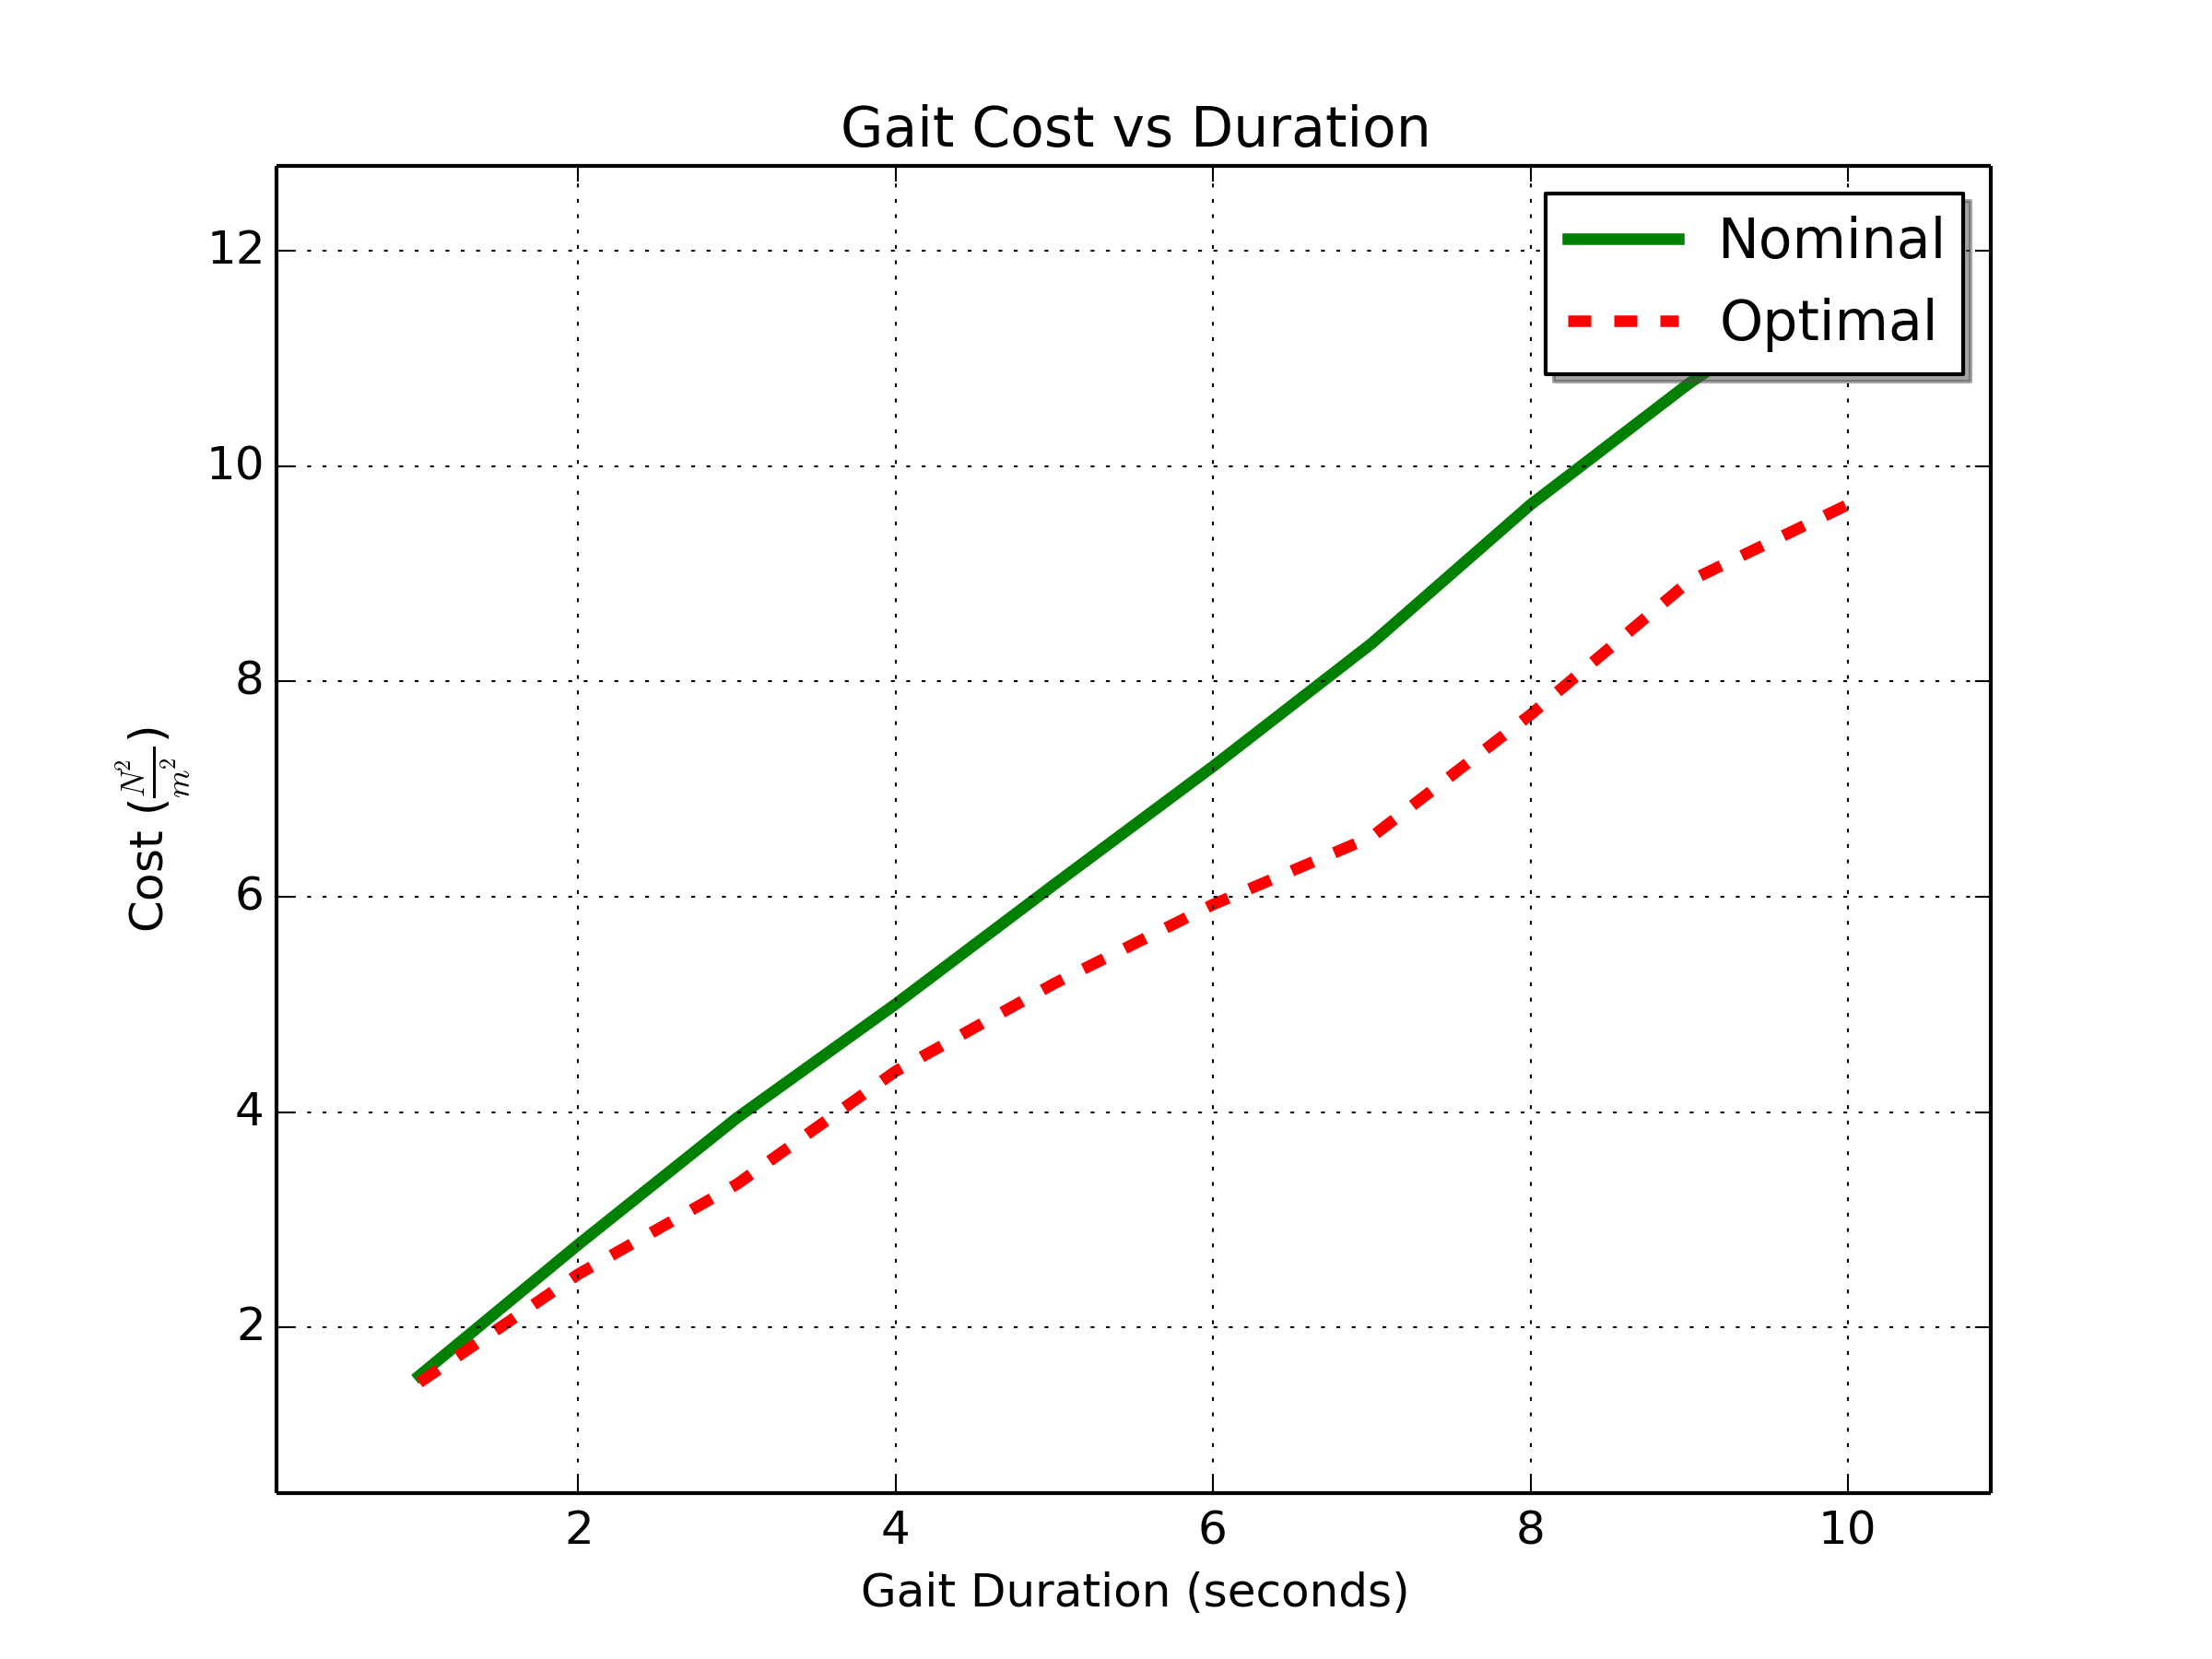
\includegraphics[width=0.5\textwidth]{crawl/cost/gait_cost_duration1.png}
  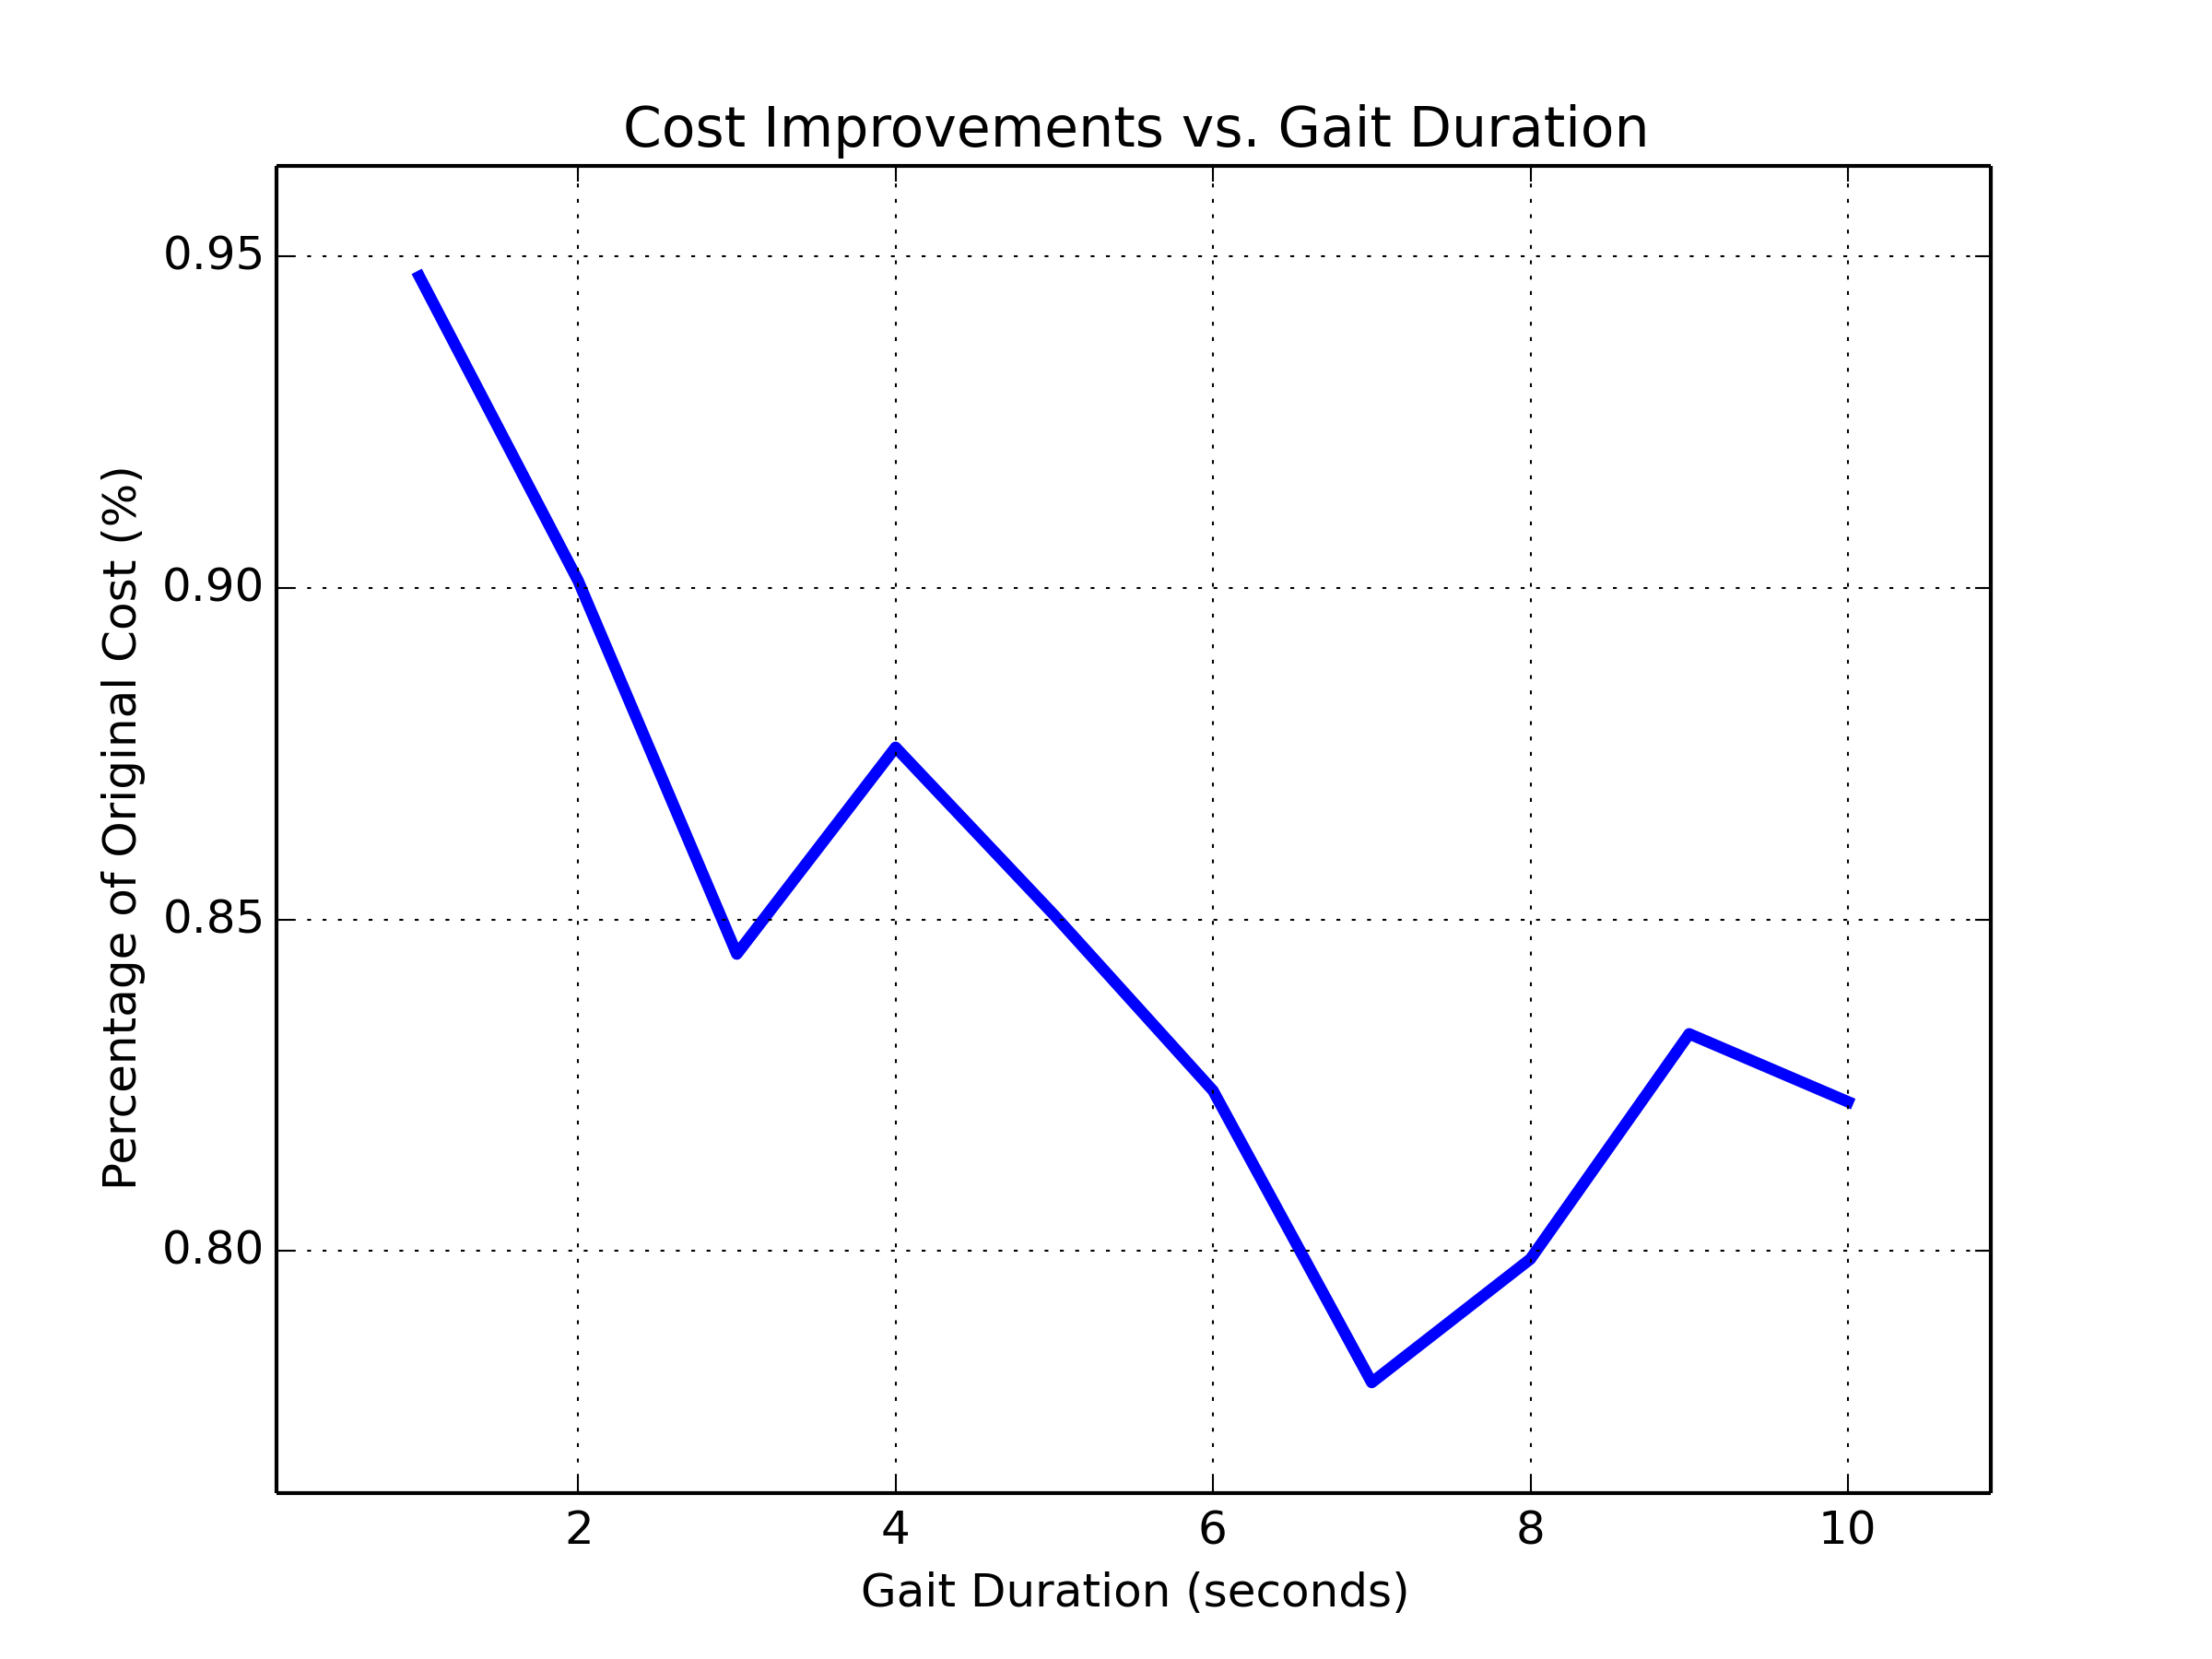
\includegraphics[width=0.5\textwidth]{crawl/cost/cost_imp_duration1.png}
  \vspace*{-0.05in}
  \caption{BLAH BLAH Things about gait cost comparisons.}
  \label{fig:cost_duration1}
  \vspace*{-0.01in}
  \vspace*{-0.05in}
\end{figure}

\begin{figure}
  \centerline{
    \includegraphics[width=0.5\textwidth]{crawl/vrep/nominal/1.png}
    \includegraphics[width=0.5\textwidth]{crawl/vrep/nominal/2.png}
  }
  \vspace*{0.05in}
  \centerline{
    \includegraphics[width=0.5\textwidth]{crawl/vrep/nominal/3.png}
    \includegraphics[width=0.5\textwidth]{crawl/vrep/nominal/4.png}
  }
  \vspace*{0.05in}
  \centerline{
    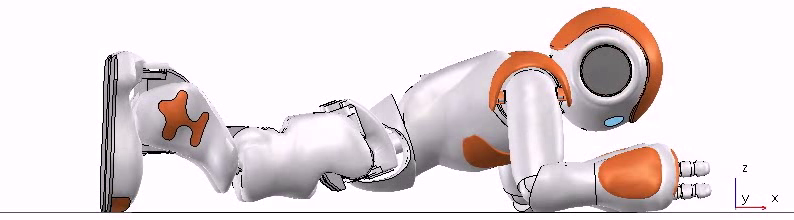
\includegraphics[width=0.5\textwidth]{crawl/vrep/nominal/5.png}
  }
  \vspace*{-0.05in}
  \caption{BLAH BLAH Simulated Nao with nominal gait.}
  \label{fig:vrep_nao_nom_gait1}
  \vspace*{-0.01in}
  \vspace*{-0.05in}
\end{figure}

\begin{figure}
  \centerline{
    \includegraphics[width=0.5\textwidth]{crawl/vrep/optimized/1.png}
    \includegraphics[width=0.5\textwidth]{crawl/vrep/optimized/2.png}
  }
  \vspace*{0.05in}
  \centerline{
    \includegraphics[width=0.5\textwidth]{crawl/vrep/optimized/3.png}
    \includegraphics[width=0.5\textwidth]{crawl/vrep/optimized/4.png}
  }
  \vspace*{0.05in}
  \centerline{
    \includegraphics[width=0.5\textwidth]{crawl/vrep/optimized/5.png}
  }
  \vspace*{-0.05in}
  \caption{BLAH BLAH Simulated Nao with optimized gait.}
  \label{fig:vrep_nao_opt_gait1}
  \vspace*{-0.01in}
  \vspace*{-0.05in}
\end{figure}

\begin{figure}
  \centerline{
    \includegraphics[width=0.5\textwidth]{crawl/pp/nominal/angle30.6_1.png}
    \includegraphics[width=0.5\textwidth]{crawl/pp/nominal/angle42_1.png}
  }
  \vspace*{0.05in}
  \centerline{
    \includegraphics[width=0.5\textwidth]{crawl/pp/nominal/angle54_1.png}
    \includegraphics[width=0.5\textwidth]{crawl/pp/nominal/angle66.6_1.png}
  }
  \vspace*{0.05in}
  \centerline{
    \includegraphics[width=0.5\textwidth]{crawl/pp/nominal/angle78_1.png}
    \includegraphics[width=0.5\textwidth]{crawl/pp/nominal/angle90_1.png}
  }
  \vspace*{-0.05in}
  \caption{BLAH BLAH Projected Profile Nao with nominal gait.}
  \label{fig:pp_nom_gait1}
  \vspace*{-0.01in}
  \vspace*{-0.05in}
\end{figure}

\begin{figure}
  \centerline{
    \includegraphics[width=0.5\textwidth]{crawl/pp/optimal/angle30_1.png}
    \includegraphics[width=0.5\textwidth]{crawl/pp/optimal/angle42.7474_1.png}
  }
  \vspace*{0.05in}
  \centerline{
    \includegraphics[width=0.5\textwidth]{crawl/pp/optimal/angle54.5496_1.png}
    \includegraphics[width=0.5\textwidth]{crawl/pp/optimal/angle66.4421_1.png}
  }
  \vspace*{0.05in}
  \centerline{
    \includegraphics[width=0.5\textwidth]{crawl/pp/optimal/angle78.1161_1.png}
    \includegraphics[width=0.5\textwidth]{crawl/pp/optimal/angle89.9428_1.png}
  }
  \vspace*{-0.05in}
  \caption{BLAH BLAH Projected Profile Nao with optimal gait.}
  \label{fig:pp_opt_gait1}
  \vspace*{-0.01in}
  \vspace*{-0.05in}
\end{figure}

PUT IN THE OPTIMIZATION COSTS (Check out the torque only ones and the torque plus indication
function costs to see what kind of influence those functions had on the optimization.)


